\chapter{Trajectory Planning - Laparoscopic tool manipulation}
\label{chapter-6}
%
Trajectory planning is executed after a desired path is generated, and consists in mapping the geometric points to specific \textbf{time points}, as well as assigning specific \textbf{velocities}, \textbf{accelerations} and \textbf{jerks}, 
in order to generate the commands needed for the robot controller to execute a smooth motion.\\

The paths that are calculated are parameterized by the path parameter $s$. As $s$ increases from $0$, the robot moves from the start configuration $q(0)$ to the goal configuration $q(1)$. 
Path planning outputs geometric information $q(s), s \in [0, 1]$, whereas the \textbf{trajectories} that are the subject of this chapter, also include \textbf{time information} $q(t), t \in [0, T]$. 
A path can be converted to a trajectory by defining a function $s(t): [0, T] \rightarrow [0, 1]$ which maps the time parameter's range to the path parameter's range. This function is also known as \textbf{time scaling} or 
\textbf{time parameterization}.The most common methodology of trajectory planning, which is also used in this thesis, is the one that is studied in the \textbf{joint angles space} also known as \textbf{configuration space}.\\

The biggest challenge in manipulating a laparoscopic tool with a robot is overcoming the \textbf{fulcrum effect} problem. This is also one of the reasons that 
robotic assisted surgery replaced the traditional laparoscopic procedures. The fulcrum effect means that the surgeon's hand motions are inverted and scaled 
with respect to the Remote Center of Motion point, which lies approximately on the center of the incision. Apart from the scaling and inversion, laparoscopic 
procedures add an additional motion constraint that demands at each time one point of the laparoscopic tool to coincide with the RCM point.\\

\section{Tool pose \& the Fulcrum Effect}
\label{section:fulcrum-effect}

\begin{center}
\begin{figure}[htbp]
\centering
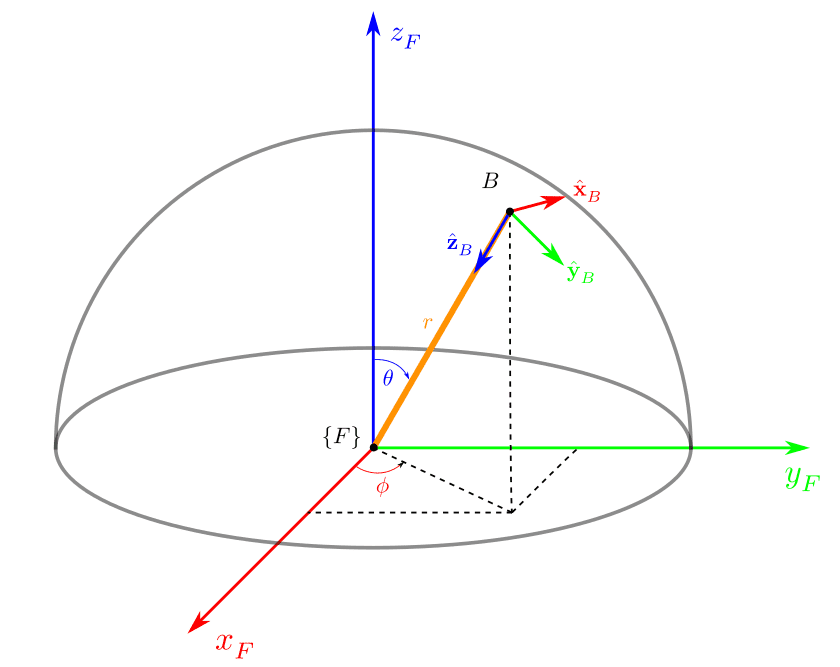
\includegraphics[width=0.7\textwidth]{images/fulcrum-space.png}\\
\caption{Tool pose at target point $B$ calculated with respect to Fulcrum's reference frame $\lbrace F \rbrace$}
\end{figure}
\end{center}

The laparoscopic tool pose is given by the position and orientation vectors at target point $B$ with respect to the coordinate frame $\lbrace F \rbrace$.
The pose is given by the following transformation matrix
\[
{}^{F}T_B = \begin{bmatrix}
{}^{F}R_B & {}^{F}\mathbf{p}^{}_B \\
\mathbf{0} & 1 \\
\end{bmatrix}
\;\; where \;\;
{}^{F}R_B = \begin{bmatrix}
\hat{\mathbf{x}}^{}_B & \hat{\mathbf{y}}^{}_B & \hat{\mathbf{z}}^{}_B \\
\end{bmatrix}
\]

\begin{equation}
\hat{\mathbf{x}}^{}_B = \hat{\mathbf{φ}} = -\sin(φ)\hat{\mathbf{x}}^{}_F + \cos(φ)\hat{\mathbf{y}}^{}_F
= \begin{bmatrix}
-\sin(φ) \\
\cos(φ) \\
0 \\
\end{bmatrix}
\end{equation}

\begin{equation}
\hat{\mathbf{y}}^{}_B = \hat{\mathbf{θ}} = \cos(θ)\cos(φ)\hat{\mathbf{x}}^{}_F + \cos(θ)\sin(φ)\hat{\mathbf{y}}^{}_F - \sin(θ)\hat{\mathbf{z}}^{}_F
= \begin{bmatrix}
\cos(θ)\cos(φ) \\
\cos(θ)\sin(φ) \\
- \sin(θ) \\
\end{bmatrix}
\end{equation}

\begin{equation}
\hat{\mathbf{z}}^{}_B = \hat{\mathbf{r}} = \sin(θ)\cos(φ)\hat{\mathbf{x}}^{}_F + \sin(θ)\sin(φ)\hat{\mathbf{y}}^{}_F + \cos(θ)\hat{\mathbf{z}}^{}_F
= \begin{bmatrix}
\sin(θ)\cos(φ) \\
\sin(θ)\sin(φ) \\
\cos(θ) \\
\end{bmatrix}
\end{equation}

The position of the point $B$ is given in spherical coordinates by:
\begin{itemize}
	\item $r=ρ$ : outside penetration of laparoscopic tool
	\item $θ=β$ : altitude angle
	\item $φ=α$ : orientation angle
\end{itemize}
thus the position with respect to the coordinate frame $\lbrace F \rbrace$ is given by
\begin{equation}
{}^{F}\mathbf{p}^{}_B = \begin{bmatrix}
ρ\sin(β)\cos(α) \\
ρ\sin(β)\sin(α) \\
ρ\cos(β) \\
\end{bmatrix} = ρ \hat{\mathbf{r}}
\end{equation}

After having calculated the $\hat{\mathbf{x}},\hat{\mathbf{y}},\hat{\mathbf{z}},\mathbf{p}$, then these are rotated according to how the tool is attached on the end-effector (e.g. in this thesis the $\hat{\mathbf{x}}$ vector 
points towards the origin of the frame, see figure \ref{robot-planner3b-line-seg}) of the robot and they are also translated (see also figure \ref{robot-planner3b-line-seg})
based on the offset between the end-effector and the tool (distance between end-effector and TCP). Note, that one can also use the $φ,θ$ angles as two of the Euler rotation angles and thus calculate the orientation 
with these angles instead of using the spherical coordinate unit vectors method above.
The final transformed goal pose must be the same as the $TCP$ point of the robot's end-effector. This means, that this pose must be converted with respect to the robot's reference frames.
\[
{}^{U}T^{}_{TCP} = {}^{U}T^{}_{B}
\]
\[
{}^{U}T^{}_{0} \; {}^{0}T^{}_{7} \; {}^{7}T^{}_{TCP} = {}^{U}T^{}_{F} \; {}^{F}T^{}_{B}
\]
\begin{equation}
{}^{0}T^{}_{7} = {}^{U}T^{-1}_{0} \; {}^{U}T^{}_{F} \; {}^{F}T^{}_{B} \; {}^{7}T^{-1}_{TCP}
\end{equation}

\begin{listing}[H]
\begin{minted}[tabsize=2,breaklines,frame=lines,framesep=2mm,baselinestretch=1.2,fontsize=\footnotesize, linenos]{matlab}
function tcp = fulcrumEffectTrajectory(P, L)
    tcp = zeros(size(P));
    for i=1:size(P)
        px = P(i,1); py = P(i,2); pz = P(i,3);
        r = sqrt(px^2+py^2+pz^2);
        th = atan2(sqrt(px^2+py^2), pz);
        phi = atan2(py, px);
        vx = [cos(th)*cos(phi); cos(th)*sin(phi); -sin(th)];
        vy = [-sin(phi); cos(phi); 0];
        vz = [-sin(th)*cos(phi); -sin(th)*sin(phi); cos(th)];
        vp = r*[sin(th)*cos(phi); sin(th)*sin(phi); cos(th)];
        T = zeros(4,4);
        R = [vx, vy, vz];
        T(1:3,1:3) = R;
        T(1:3,4) = vp;
        T(4,4) = 1;
        Td = eye(4);
        Td(1:3,4) = (r-L)/r*vp;
        tcp_point = Td*inv(T)*[P(i,:).'; 1];
        tcp(i,:) = tcp_point(1:3).';
    end
end
\end{minted}
\caption{Fulcrum Effect transformation of a trajectory, in MATLAB}
\label{code:fulcrum_effect_traj_matlab}
\end{listing}


\section{Trajectory planning in cartesian coordinates}
\label{section:pivot-motions}

On this section, some basic pivoting trajectories around the fulcrum point, are presented. In all of the following three example pivoting motions, we have made 
the assumption that the position and orientation of the ${F}$ reference frame is precisely known, which is however not applicable in real-life scenarios. The trajectories 
presented in this section are planned in cartesian coordinates or also known as \textbf{Task space}.

\underline{Advantages of planning in Task Space}
\begin{itemize}
\item Since the interpolation of the path points is in task space, then the planned motion is \textbf{more predictable}.
\item It is easier to design trajectories which are \textbf{better in avoiding obstacles and handling collisions}.
\end{itemize}

\underline{Disadvantages of planning in Task Space}
\begin{itemize}
\item \textbf{Planning and execution are significantly slower}, because for each interpolation point in task space the Inverse Kinematics problem must be solved. This issue is
even more problematic when the IK problem is not solved with analytical equations but numerically using optimization techniques.
\item A smooth trajectory in task space is not necessarily smooth in Joint Space (see figure \ref{interpolation-accuracy}).
\end{itemize}

\begin{center}
\begin{figure}[htbp]
\centering
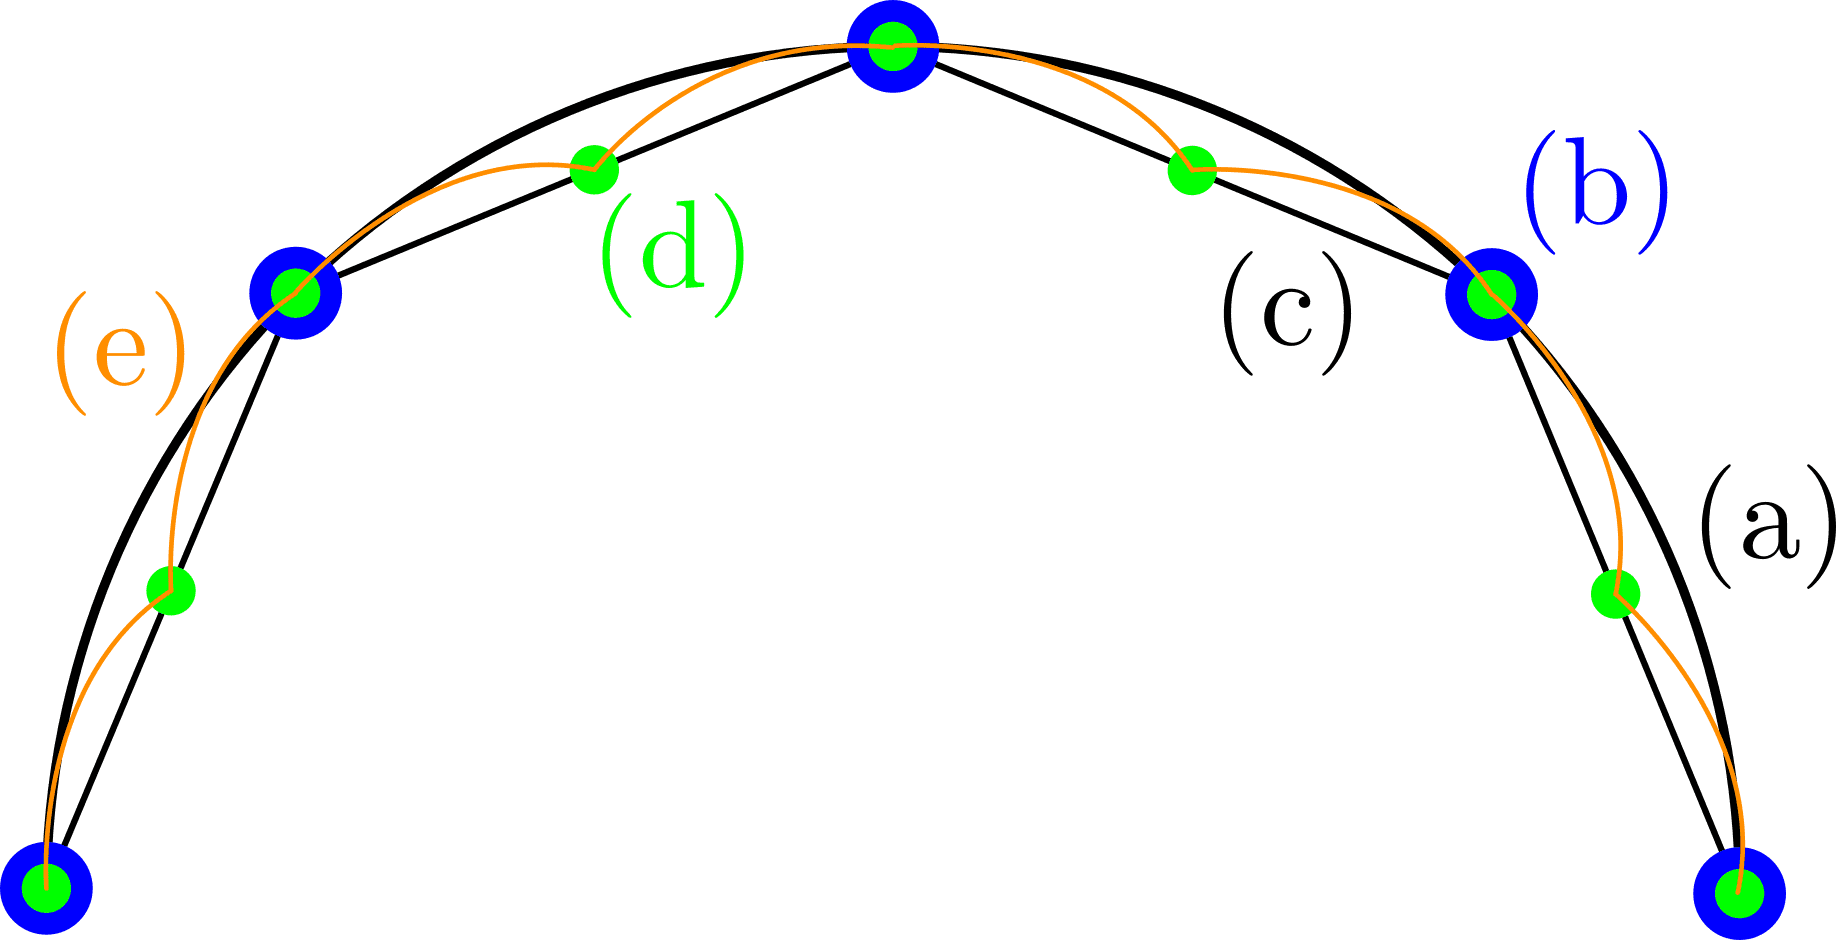
\includegraphics[width=0.5\textwidth]{images/interpolation-accuracy.png}\\
\caption{Path/trajectory interpolation done at two stages. (a) the initial desired circular trajectory, (b) sample waypoints that will approximate the circle and shape a polygon, (c) the line segments connecting the waypoints and which the robot must theoretically follow exactly, (d) lower-level interpolation of the line segments (made by MoveIt in ROS or by the robot's controller when executing PtP), (e) the actual trajectory that 
the robot will follow}
\label{interpolation-accuracy}
\end{figure}
\end{center}

\subsection{Circular trajectory of tool tip}

\begin{center}
\begin{figure}[htbp]
\centering
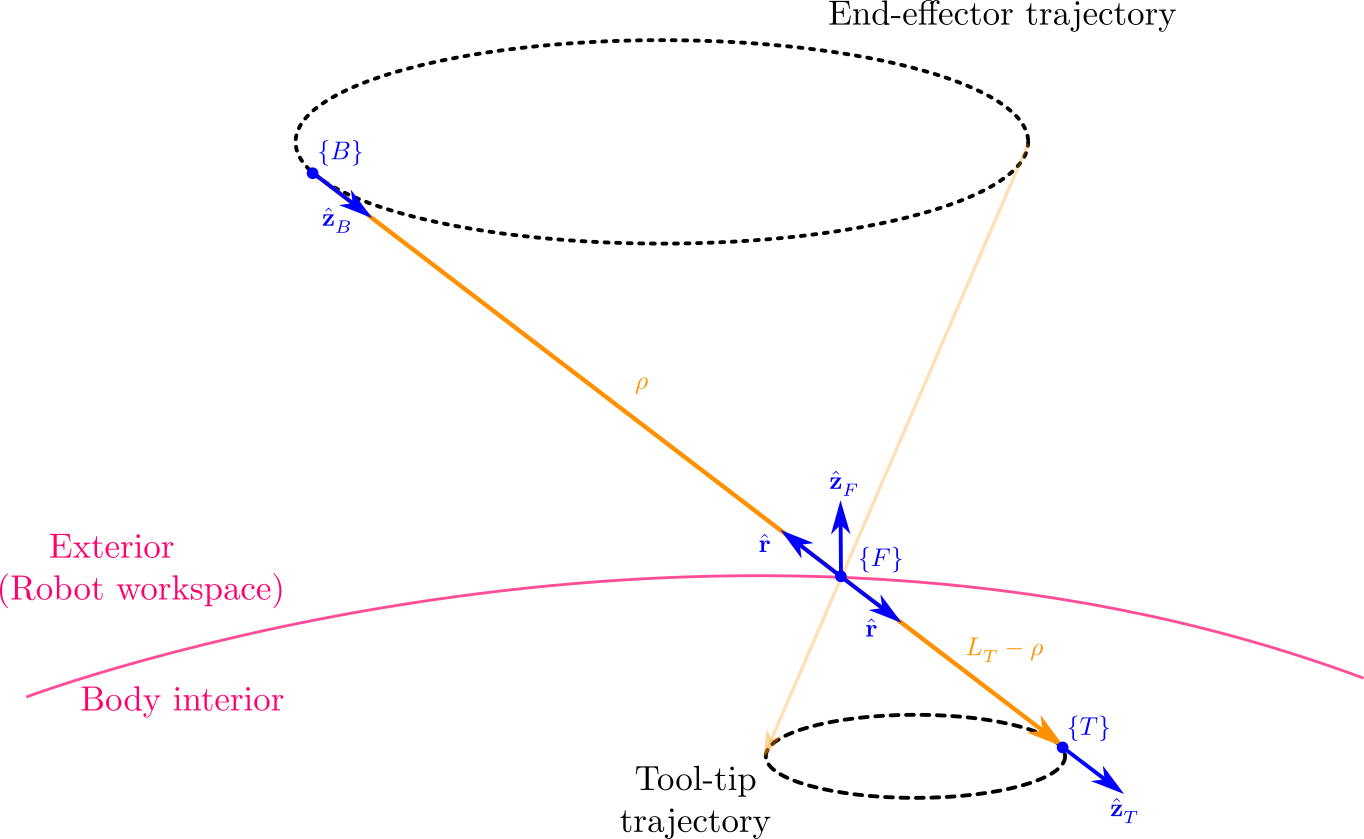
\includegraphics[width=0.7\textwidth]{images/circular-trajectory-wrt-fulcrum.png}\\
\caption{Circular trajectory of tool tip with respect to Fulcrum reference frame}
\end{figure}
\end{center}

To generate a circular trajectory for the pivot movement we must specify the center of the circle and a vector whose magnitude is the radius of the circle and it’s direction gives the orientation of the plane that the circle lies at. The simplest case of a circular trajectory, where the circle lies in a plane parallel to the xy plane.

We first consider the motion of the laparoscopic tool tip on a circle parallel to a z-plane, with respect to the $\lbrace F \rbrace$ coordinate frame.
\begin{equation}
(x^{}_{F} - x^{}_{F0})^2 + (y^{}_{F} - y^{}_{F0})^2 = r_0^2, \;\; z^{}_{F} = z^{}_{F0}
\end{equation}
It is more convenient to express trajectories in a parametric form,
\begin{equation}
\label{circle-z-plane-traj}
\begin{cases}
x^{}_{F} = r_0\cos(2πs) + x^{}_{F0} \\
y^{}_{F} = r_0\sin(2πs) + y^{}_{F0} \\
z^{}_{F} = z^{}_{F0}
\end{cases} ,
\;\;
s \in [0, 1]
\end{equation}

After having calculated the cartesian coordinates we can calculate the spherical coordinates as 
\begin{equation}
\label{eqns:cartesian-to-spherical}
\begin{cases}
r = \sqrt{x^{2}_{F} + y^{2}_{F} + z^{2}_{F}} \\
θ = atan2 \left( \sqrt{x^{2}_{F} + y^{2}_{F}}, z^{}_{F} \right) \\
φ = atan2(y^{}_{F}, x^{}_{F})
\end{cases}
\end{equation}

\begin{center}
\begin{figure}[htbp]
\centering
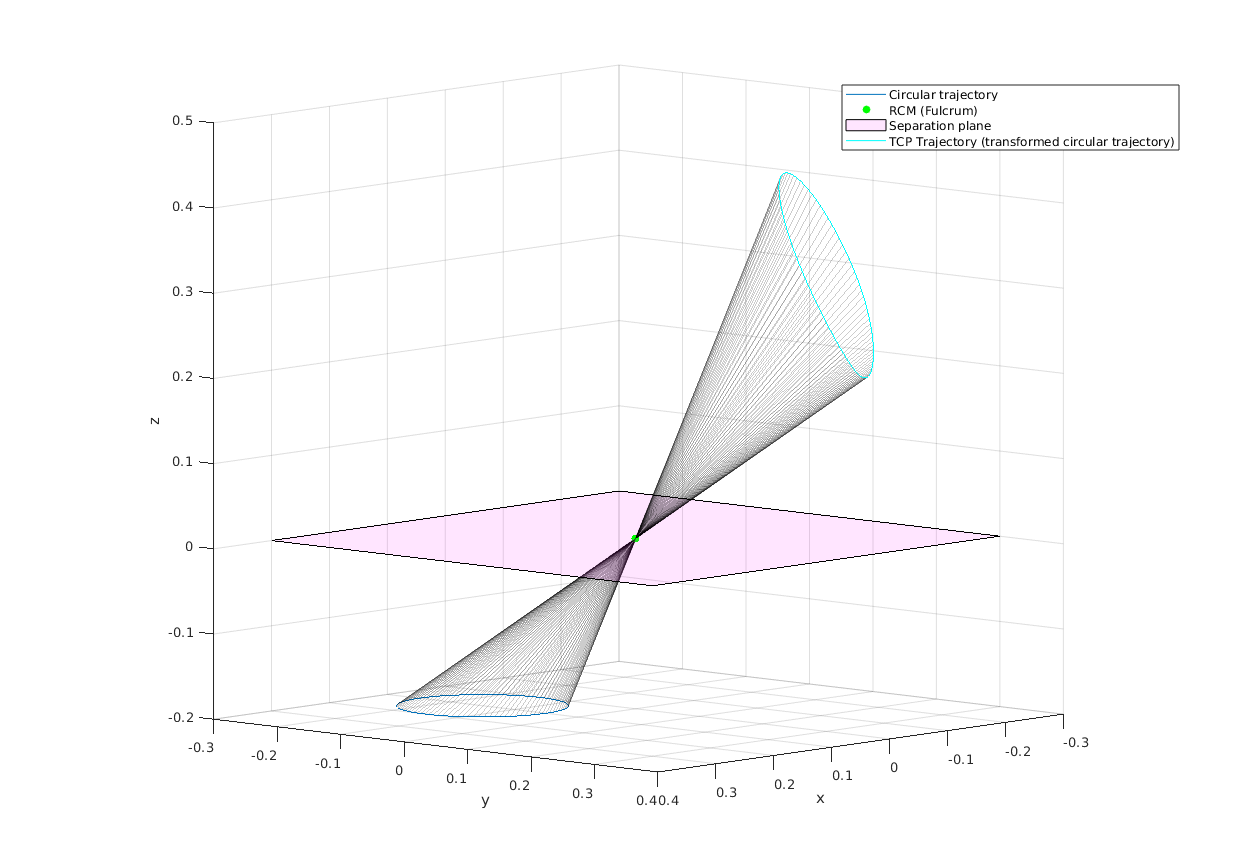
\includegraphics[width=0.7\textwidth]{images/rcm_trajectories/rcm_circle_traj.png}\\
\caption{Circular trajectory of tool tip with respect to Fulcrum reference frame and it's transformation via the Fulcrum Effect}
\end{figure}
\end{center}

Although the equations \ref{circle-z-plane-traj} are very simple to calculate, it is more often the case that the circular trajectory will lie on an arbitrary plane that will not be parallel to the z-plane. This means 
that the equations \ref{circle-z-plane-traj} must first be transformed inside the task space (with the desired rotation and translation) and then these transformed equations should be used as an input to the 
Fulcrum Effect transformation.

\begin{center}
\begin{figure}[htbp]
\centering
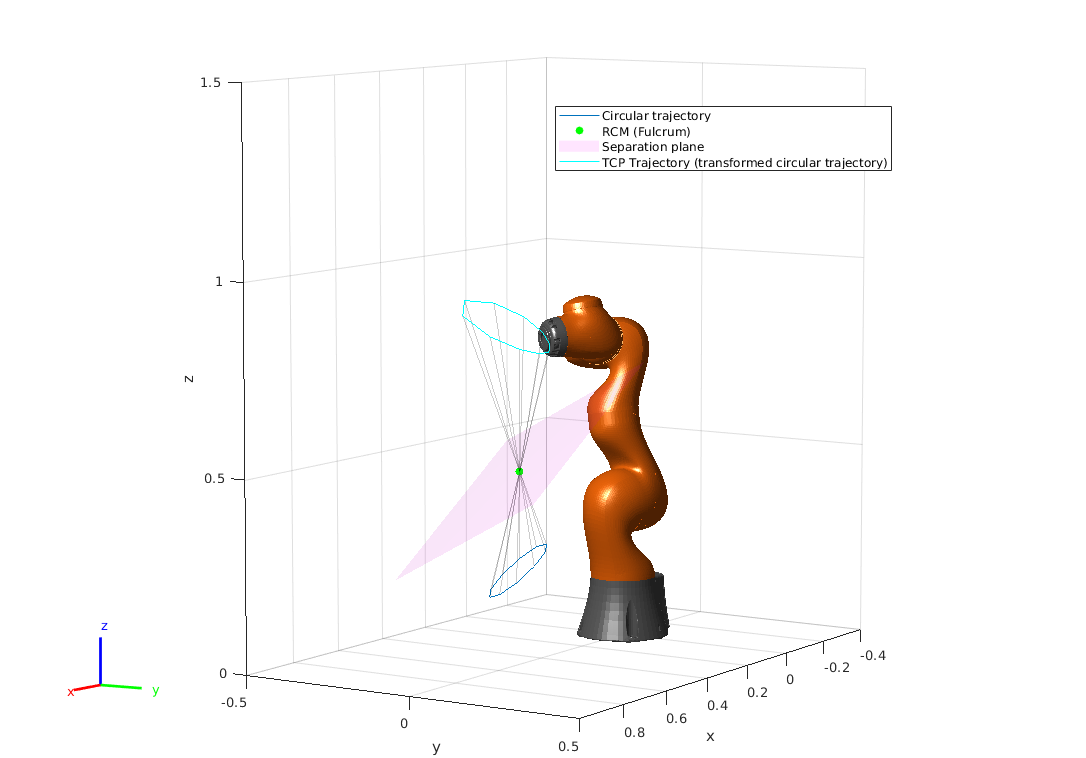
\includegraphics[width=0.7\textwidth]{images/rcm_trajectories/robot-pose-random-rcm-circle-traj.png}\\
\caption{Circular trajectory that lies on an a plane of arbitrary orientation with respect to the fulcrum point}
\end{figure}
\end{center}

\subsection{Circular arc trajectory of tool tip}

To generate a circular arc trajectory for a pivot motion we must specify the same parameters as 
in the circular trajectory as well as the length of the arc or the total angle $φ$ of the arc section. Another parameter has more significance in circular arc trajectories that plain circles is the phase of the arc. This initial phase can be expressed as either an angle $φ_0$ added to the arguments of 
sine and cosine functions or it can be expressed as $s$ values that have as initial value different from $0$. The parametric equations for a circular arc are:

\begin{equation}
\begin{cases}
x^{}_{F} = r_0\cos(2πs + φ_0) + x^{}_{F0} \\
y^{}_{F} = r_0\sin(2πs + φ_0) + y^{}_{F0} \\
z^{}_{F} = z^{}_{F0}
\end{cases} ,
\;\;
s \in \left[ 0, \frac{φ}{2π} \right]
\end{equation}

\begin{center}
\begin{figure}[htbp]
\centering
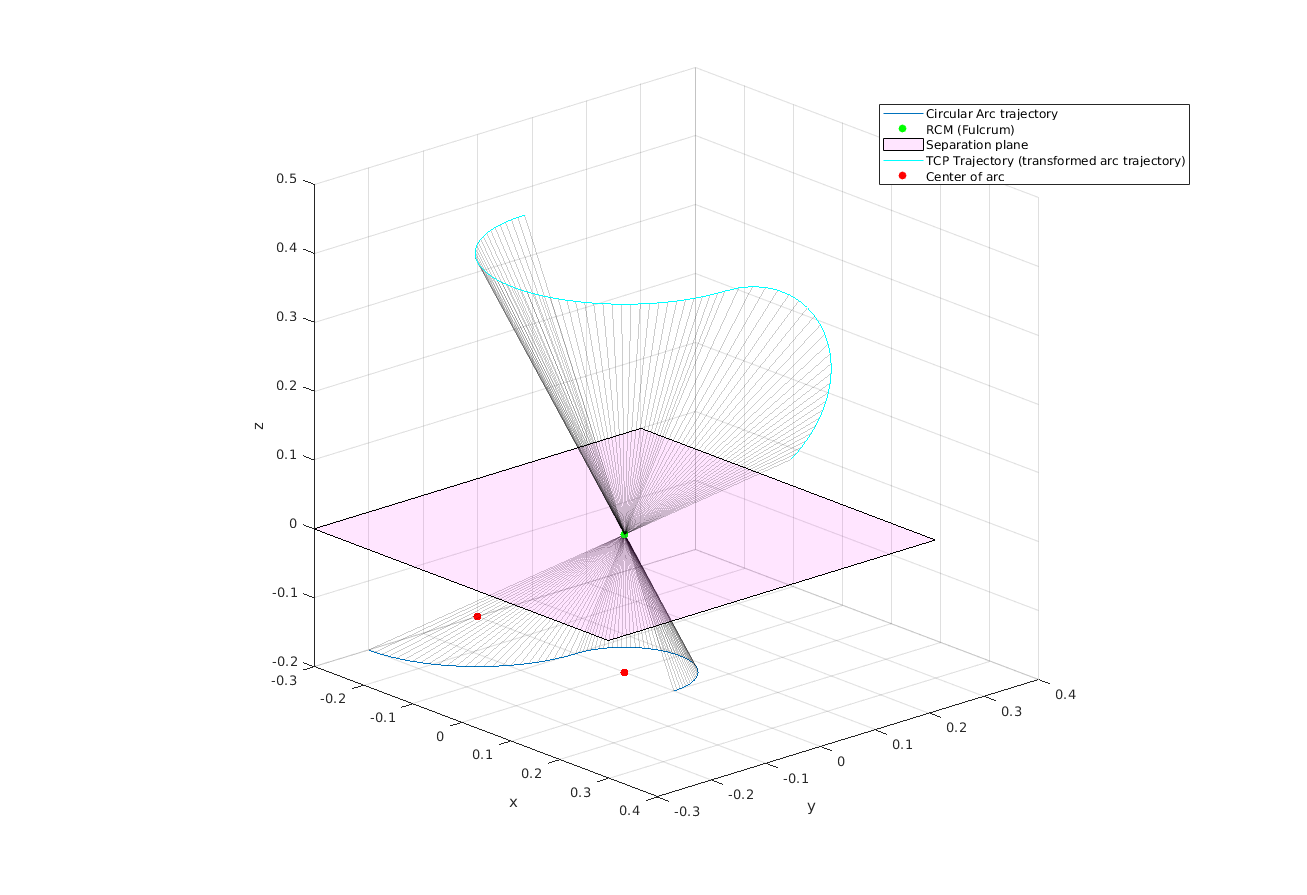
\includegraphics[width=0.7\textwidth]{images/rcm_trajectories/rcm_arcs_traj.png}\\
\caption{Circular arc trajectory of tool tip with respect to Fulcrum reference frame and it's transformation via the Fulcrum Effect. In this trajectory 2 circular arcs are used}
\end{figure}
\end{center}

\subsection{Helical trajectory of tool tip}

The helical trajectory is another useful trajectory that was studied in this thesis. The importance of this trajectory lies in the fact that the helical movement of the surgical tool can be considered as an ideal 
approximation of a suturing trajectory, a very common task in surgery which is extensively studied and researched in surgery robotics. A helical trajectory can be expressed by the following parametric equations:

\begin{equation}
\begin{cases}
x^{}_{F} = r_0\cos(2πs) + x^{}_{F0} \\
y^{}_{F} = r_0\sin(2πs) + y^{}_{F0} \\
z^{}_{F} = \pm βs
\end{cases}
\end{equation}

where $s \in \left[ 0, τ \right]$ expresses the range along the trajectory, $τ$ the cycles, and $β/r_0$ is the slope (or also known as the pitch which is given by $2πβ$)

\begin{center}
\begin{figure}[htbp]
\centering
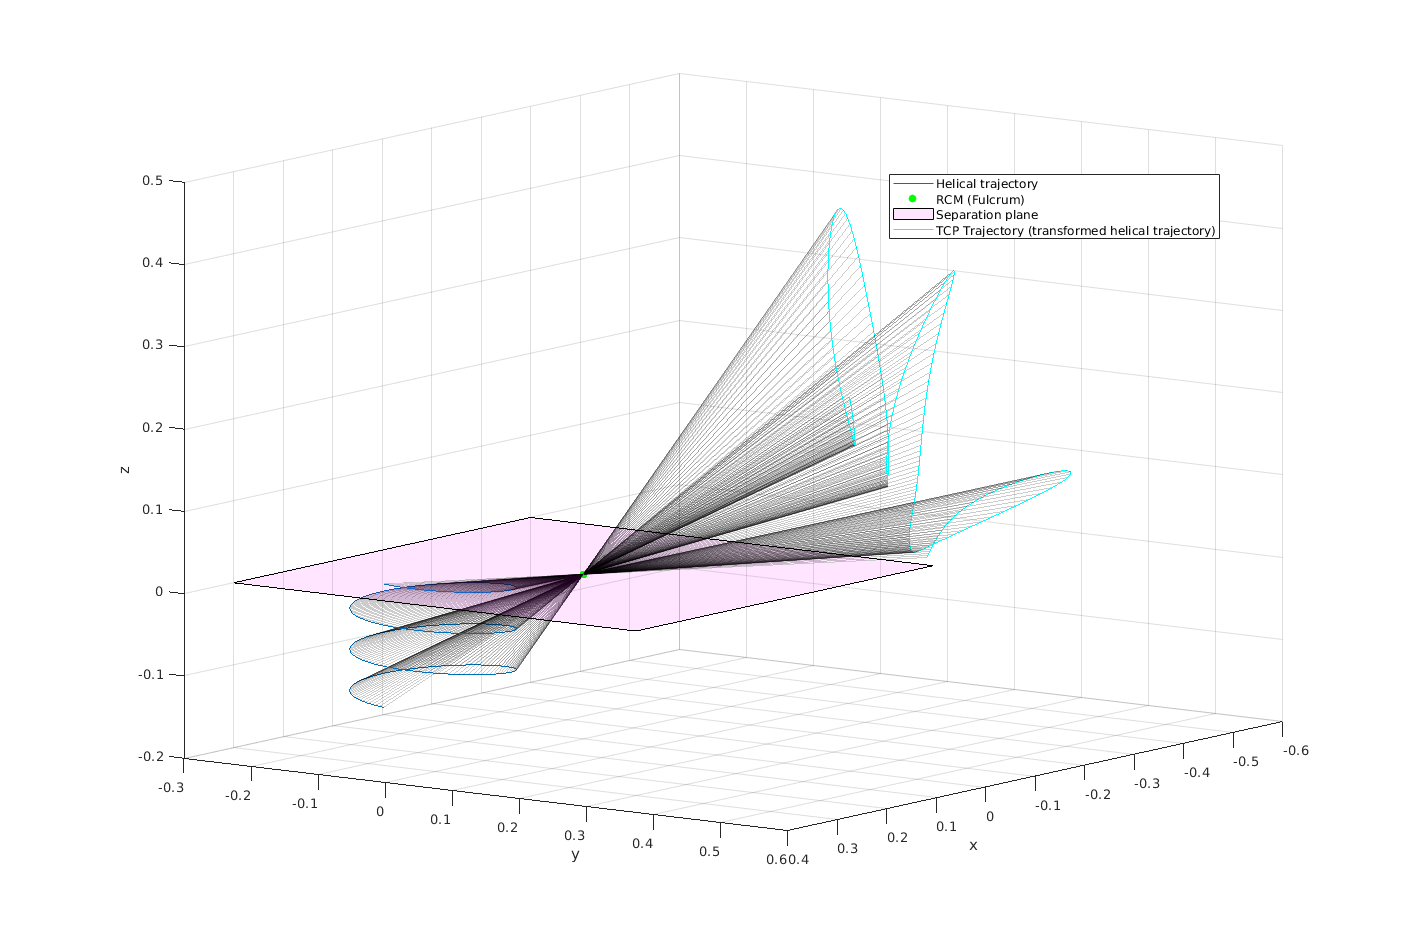
\includegraphics[width=0.7\textwidth]{images/rcm_trajectories/rcm_helical_traj.png}\\
\caption{Helical trajectory of tool tip with respect to Fulcrum reference frame and it's transformation via the Fulcrum Effect}
\end{figure}
\end{center}

\subsection{Line segment trajectory of tool tip}

\begin{center}
\begin{figure}[htbp]
\centering
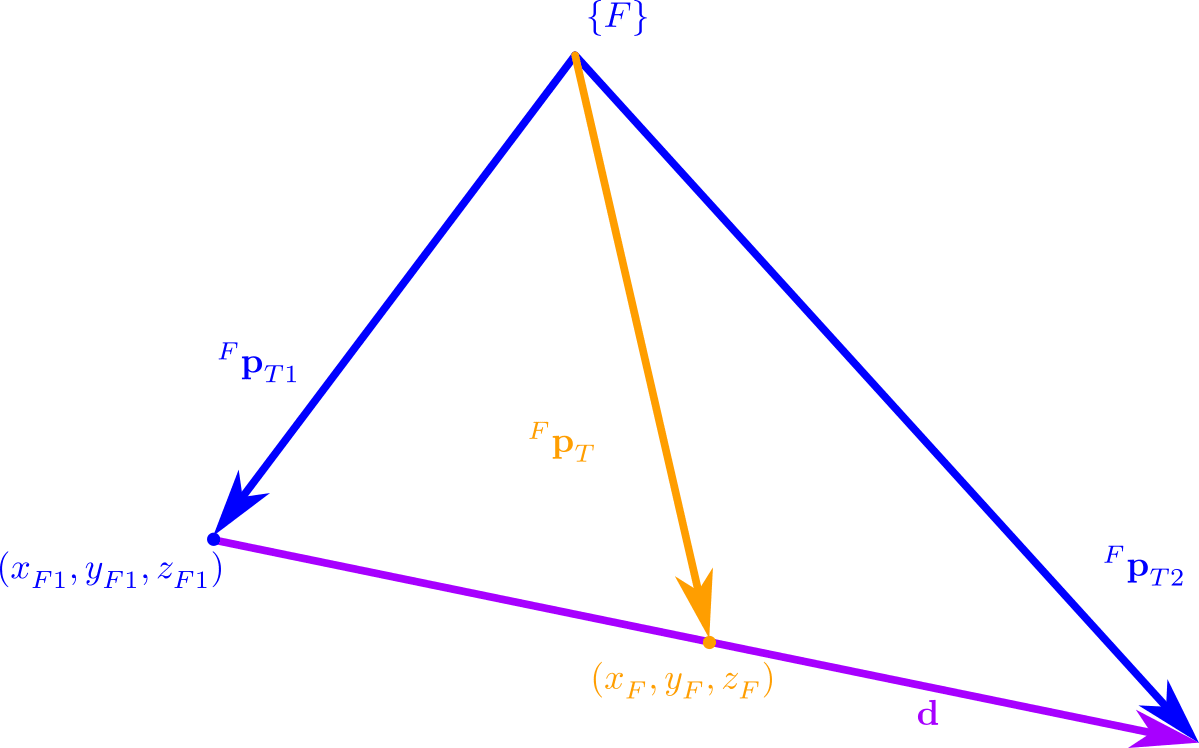
\includegraphics[width=0.7\textwidth]{images/line-segment-trajectory-wrt-fulcrum.png}\\
\caption{Line segment trajectory of tool tip with respect to Fulcrum reference frame}
\end{figure}
\end{center}
\[
\mathbf{d} = {}^{F}\mathbf{p}^{}_{T2} - {}^{F}\mathbf{p}^{}_{T1} = [l, m, n]^\top
\]
\[
{}^{F}\mathbf{p}^{}_{T} = [x^{}_{F}, y^{}_{F}, z^{}_{F}]^\top
\]
\[
{}^{F}\mathbf{p}^{}_{T} = {}^{F}\mathbf{p}^{}_{T1} + s\mathbf{d}
\]
\[
s = \frac{x^{}_{F} - x^{}_{F1}}{l} = \frac{y^{}_{F} - y^{}_{F1}}{m} = \frac{z^{}_{F} - z^{}_{F1}}{n} \;\; s \in [0, 1]
\]

\begin{equation}
\begin{cases}
x^{}_{F} = sl + x^{}_{F1} = (1-s)x^{}_{F1} + sx^{}_{F2} \\
y^{}_{F} = sm + y^{}_{F1} = (1-s)y^{}_{F1} + sy^{}_{F2} \\
z^{}_{F} = sn + z^{}_{F1} = (1-s)z^{}_{F1} + sz^{}_{F2}
\end{cases}
\end{equation}

After having calculated the cartesian coordinates we can calculate the spherical coordinates using the \ref{eqns:cartesian-to-spherical} equations.

\begin{center}
\begin{figure}[htbp]
\centering
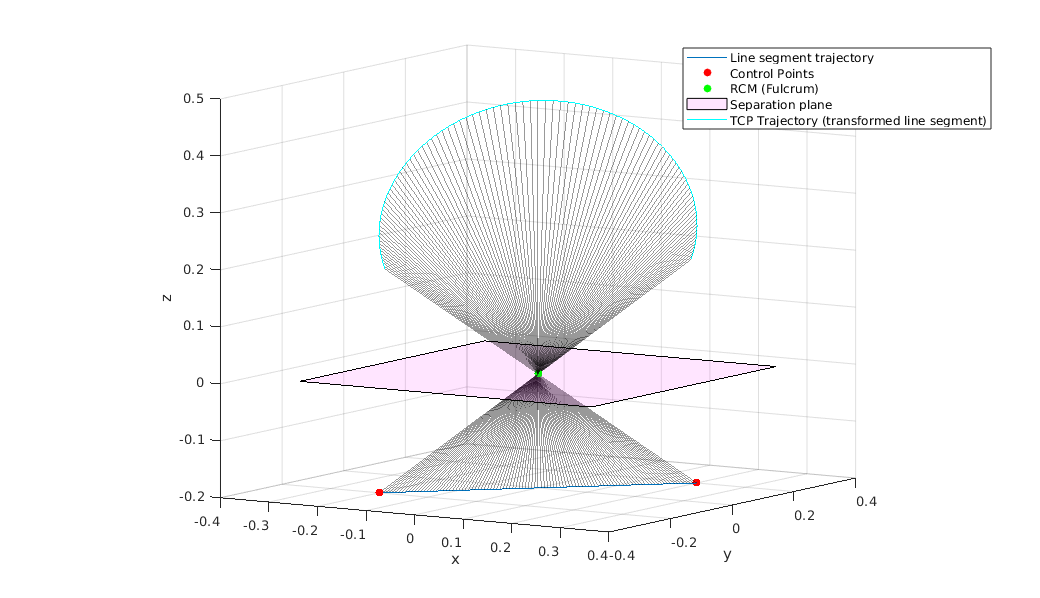
\includegraphics[width=0.7\textwidth]{images/rcm_trajectories/rcm_lineseg_traj.png}\\
\caption{A Line segment trajectory and its transformation via the Fulcrum Effect}
\end{figure}
\end{center}

The line segment trajectory of tool tip, as analysed above, \textbf{should not be confused with the} computeCartesianPath method provided by ROS MoveIt library that can be used to create line segment 
trajectories. This method produces line segment trajectories for the end effector of the robot which are not transformed as line segments via the Fulcrum Effect.

\subsection{Cubic Spline trajectory of tool tip}
\label{section:cubic-spline}

A useful mathematical tool to construct a smooth curve that visits every point from a given set of waypoints are \textbf{cubic splines}. A cubic spline is 
constructed using smaller curves that are described by a polynomial of 3rd order. Let $\left\lbrace \mathbf{P}_0, \mathbf{P}_1, \ldots , \mathbf{P}_n \right\rbrace$ 
be a set of waypoints, where each point has coordinates $\mathbf{P}_i = [x_i, y_i, z_i]^\top$. Then between each 2 points a cubic 
polynomial can be constructed (one for each coordinate, 3 in total). The following equations are for the $x$-coordinate and in the exact same way one can 
calculate the cubic polynomials for the $y,z$ coordinates as well. For each pair of waypoints we want to calculate the following cubic polynomial
\begin{equation}
\label{cubic-polynomial}
x_i(s) = a_i(s-s_i)^3 + b_i(s-s_i)^2 + c_i(s-s_i) + d_i, \hspace{3em} s_i \leqslant s \leqslant s_{i+1}
\end{equation}

The polynomial in equation \ref{cubic-polynomial} has four unknowns which means that four additional equations are needed to get a unique solution and fully 
define the polynomial. These equations can be formed using the boundary conditions for the first and last point of each curve.
\begin{equation}
x_i(s_i) = x_i
\end{equation}
\begin{equation}
x_i(s_{i+1}) = x_{i+1}
\end{equation}
\begin{equation}
\dot{x}_i(s_i) = \dot{x}_i
\end{equation}
\begin{equation}
\dot{x}_i(s_{i+1}) = \dot{x}_{i+1}
\end{equation}

First we solve for $c_i$ and $d_i$, which can easily be calculated as follows
\begin{equation}
\label{di-eq}
d_i = x_i(s_i) = x_i
\end{equation}
and by taking the derivative of \ref{cubic-polynomial}, we can calculate $c_i$
\begin{equation}
\label{cubic-polynomial-first-derivative}
\dot{x}_i(s_i) = 3a_i(s-s_i)^2 + 2b_i(s-s_i) + c_i
\end{equation}
\begin{equation}
\label{ci-eq}
c_i = \dot{x}_i(s_i) = \dot{x}_i
\end{equation}

By substituting $s = s_{i+1}$ in \ref{cubic-polynomial} and \ref{cubic-polynomial-first-derivative}, by using equations \ref{ci-eq}, \ref{di-eq} and if 
we set $σ = s_{i+1}-s_i$ for brevity, we get the following two equations
\begin{equation}
\label{xi1}
x_{i+1} = x_i(s_{i+1}) = a_i σ^3 + b_i σ^2 + c_i σ + x_i
\end{equation}
and
\begin{equation}
\label{xdi1}
\dot{x}_{i+1} = \dot{x}_i(s_{i+1}) = 3a_i σ^2 + 2b_i σ + \dot{x}_i
\end{equation}

By multiplying \ref{xdi1} by $σ$ and \ref{xi1} by $-3$ and add them together we get
\[
\dot{x}_{i+1}σ - 3x_{i+1} = -b_iσ^2 -2\dot{x}_iσ - 3x_i
\]
\begin{equation}
b_i = \frac{1}{σ^2} (3x_{i+1} -3x_i - \dot{x}_{i+1}σ - 2\dot{x}_iσ)
\end{equation}

Similarly, by multiplying \ref{xdi1} by $σ$ and \ref{xi1} by $-2$ and add them together we get
\[
\dot{x}_{i+1}σ - 2x_{i+1} = a_iσ^3 -\dot{x}_iσ - 2x_i
\]
\begin{equation}
a_i = \frac{1}{σ^3} (\dot{x}_{i+1}σ - 2x_{i+1} + \dot{x}_iσ +2x_i)
\end{equation}

\begin{center}
\begin{figure}[htbp]
\centering
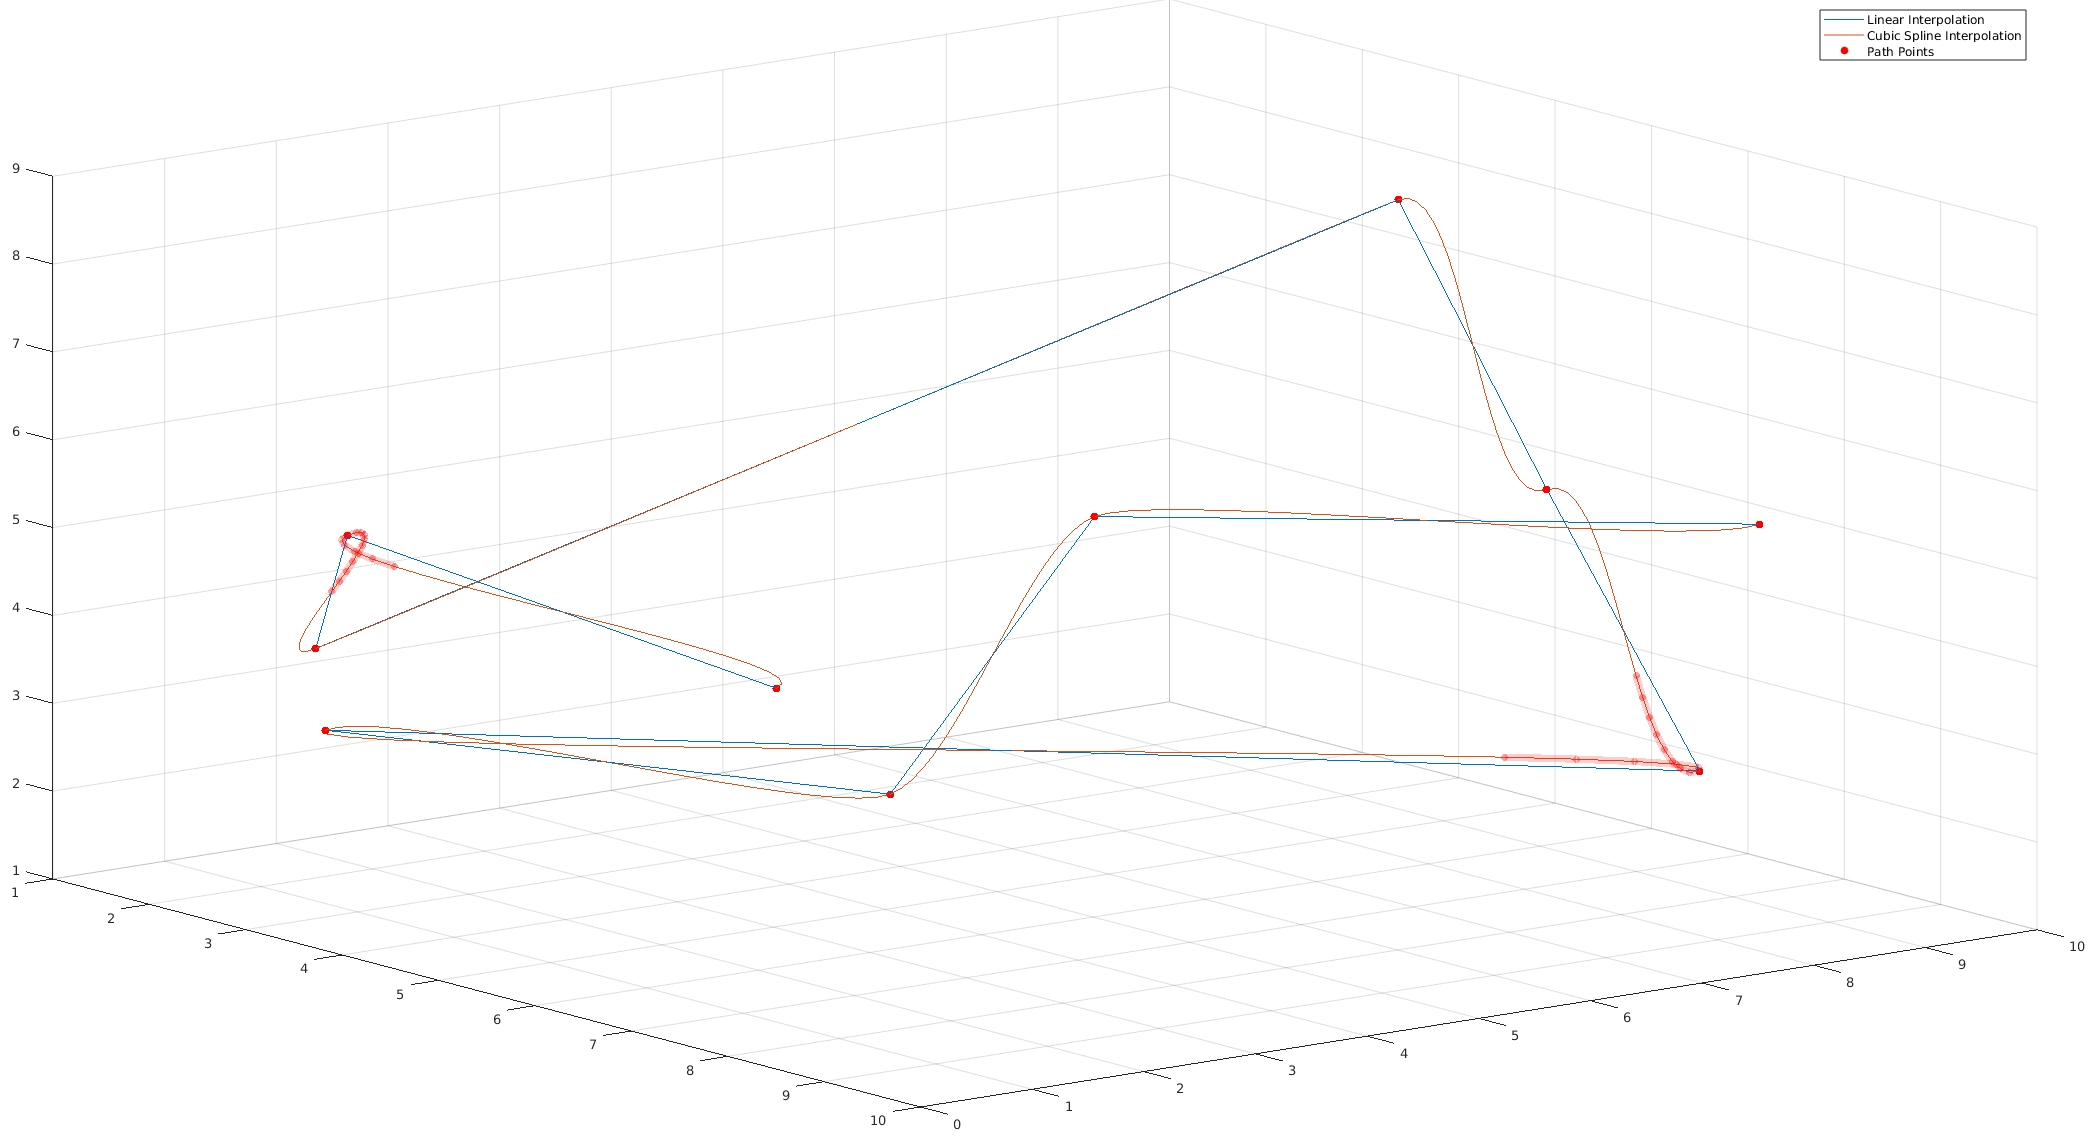
\includegraphics[width=0.7\textwidth]{images/cubic-spline-path1.png}\\
\caption{Cubic Spline curve with 10 waypoints} 
\label{cubic-spline-explanation}
\end{figure}
\end{center}

\begin{center}
\begin{figure}[htbp]
\centering
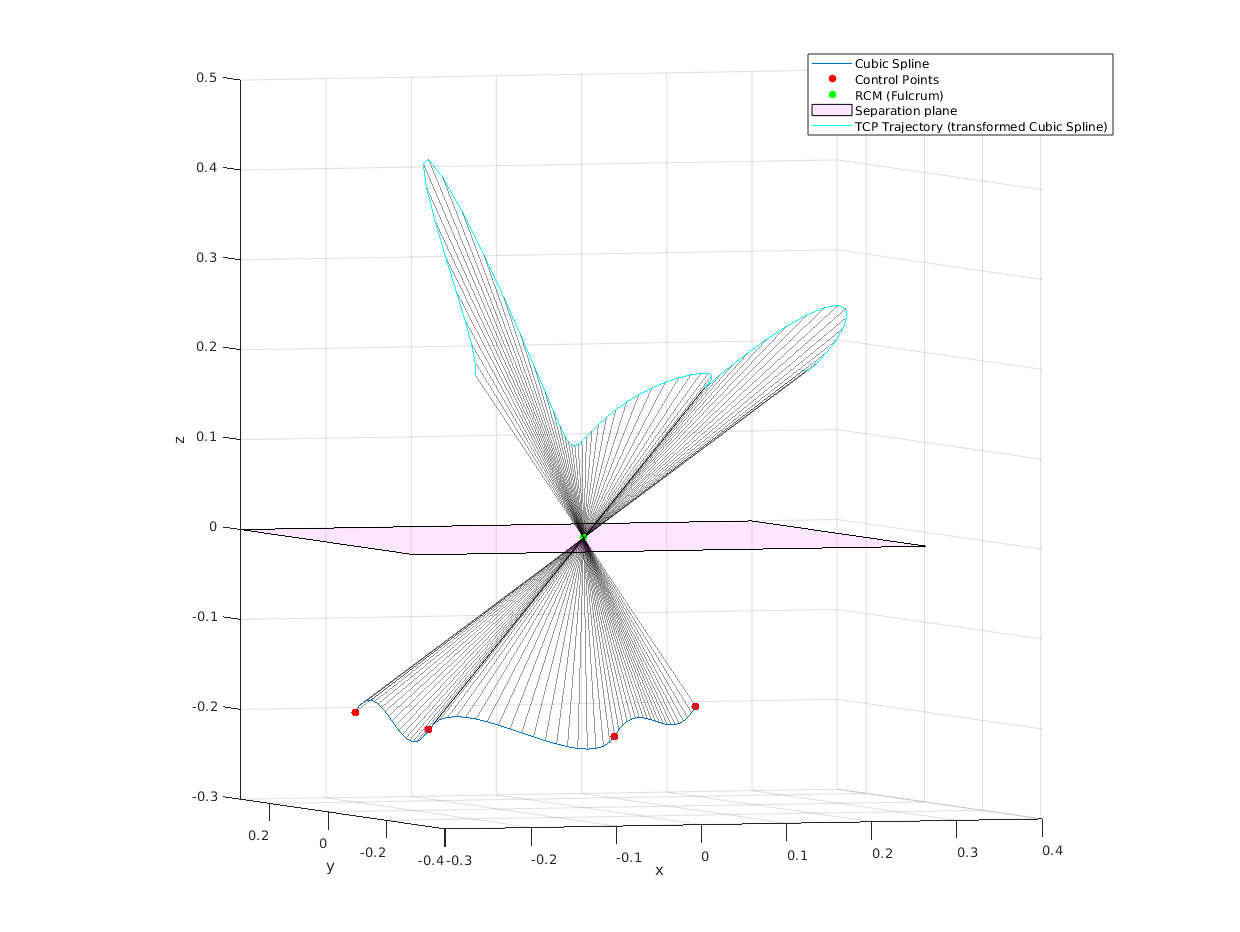
\includegraphics[width=0.7\textwidth]{images/rcm_trajectories/rcm_cubic_traj.png}\\
\caption{A Cubic Spline trajectory and it's transformation via the Fulcrum Effect}
\end{figure}
\end{center}


\subsection{B-Spline trajectory of tool tip}
\label{section:b-spline}

The \textbf{B-Splines} are smooth curves which are constructed from \textbf{B\'ezier} curves. A B\'ezier curve is a parametric smooth curve and is a $k$-th order interpolation of $k+1$ control points.

\begin{center}
\begin{figure}[htbp]
\centering
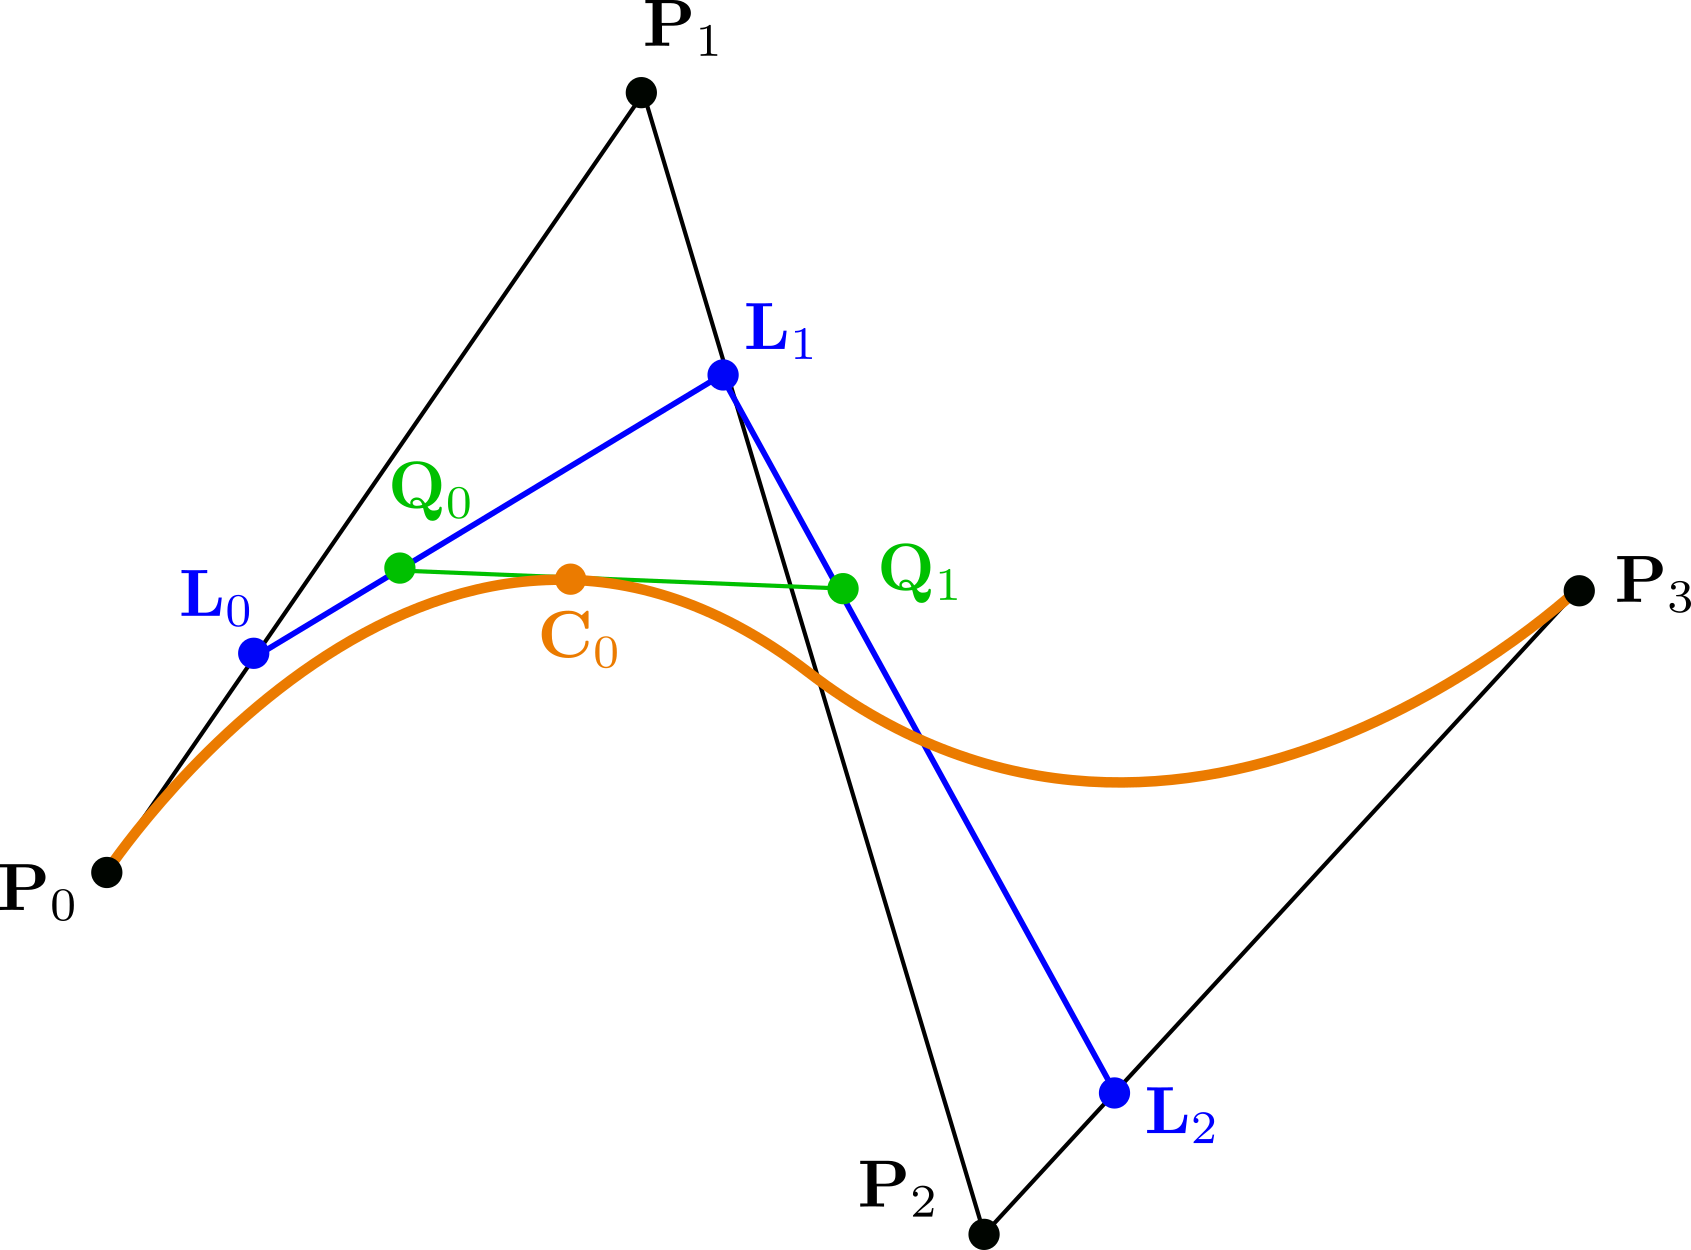
\includegraphics[width=0.5\textwidth]{images/bezier-curve.png}\\
\caption{Cubic B\'ezier curve calculated using cubic interpolation of 4 control points} 
\end{figure}
\end{center}

We first calculate the linear interpolation of the control points
\begin{equation}
\mathbf{L}_0(s) = (1-s)\mathbf{P}_0 + s\mathbf{P}_1
\end{equation}
\[
\mathbf{L}_1(s) = (1-s)\mathbf{P}_1 + s\mathbf{P}_2
\]
\[
\mathbf{L}_2(s) = (1-s)\mathbf{P}_2 + s\mathbf{P}_3
\]
The next step is to calculate the quadratic interpolation of the control points or equivalently, the linear interpolation of the previously calculated points $\mathbf{L}_0,\mathbf{L}_1,\mathbf{L}_2$
\[
\mathbf{Q}_0(s) = (1-s)\mathbf{L}_0(s) + s\mathbf{L}_1(s)
\]
\begin{equation}
\mathbf{Q}_0(s) = (1-s)^2\mathbf{P}_0 + 2(1-s)s\mathbf{P}_1 + s^2\mathbf{P}_2
\end{equation}
\[
\mathbf{Q}_1(s) = (1-s)^2\mathbf{P}_1 + 2(1-s)s\mathbf{P}_2 + s^2\mathbf{P}_3
\]
Similarly for the last step, we calculate the cubic interpolation of the control points or equivalently, the linear interpolation of the previously calculated points $\mathbf{Q}_0,\mathbf{Q}_1$
\[
\mathbf{C}_0(s) = (1-s)\mathbf{Q}_0(s) + s\mathbf{Q}_1(s)
\]
\begin{equation}
\mathbf{C}_0(s) = (1-s)^3\mathbf{P}_0 +3(1-s)^2 s\mathbf{P}_1 + 3(1-s)s^2\mathbf{P}_2 + s^3\mathbf{P}_3
\end{equation}

The cubic B\'ezier curve can also be calculated using the following more compact equation, in matrix form
\begin{equation}
\mathbf{C}_0(s) = \begin{bmatrix} \mathbf{P}_0 & \mathbf{P}_1 & \mathbf{P}_2 & \mathbf{P}_3 \end{bmatrix} 
\begin{bmatrix} 
-1 & 3 & -3 & 1 \\
3 & -6 & 3 & 0 \\
-3 & 3 & 0 & 0 \\
1 & 0 & 0 & 0
\end{bmatrix}
\begin{bmatrix}
s^3 \\ s^2 \\ s \\ 1
\end{bmatrix}
\end{equation}

\begin{center}
\begin{figure}[htbp]
\centering
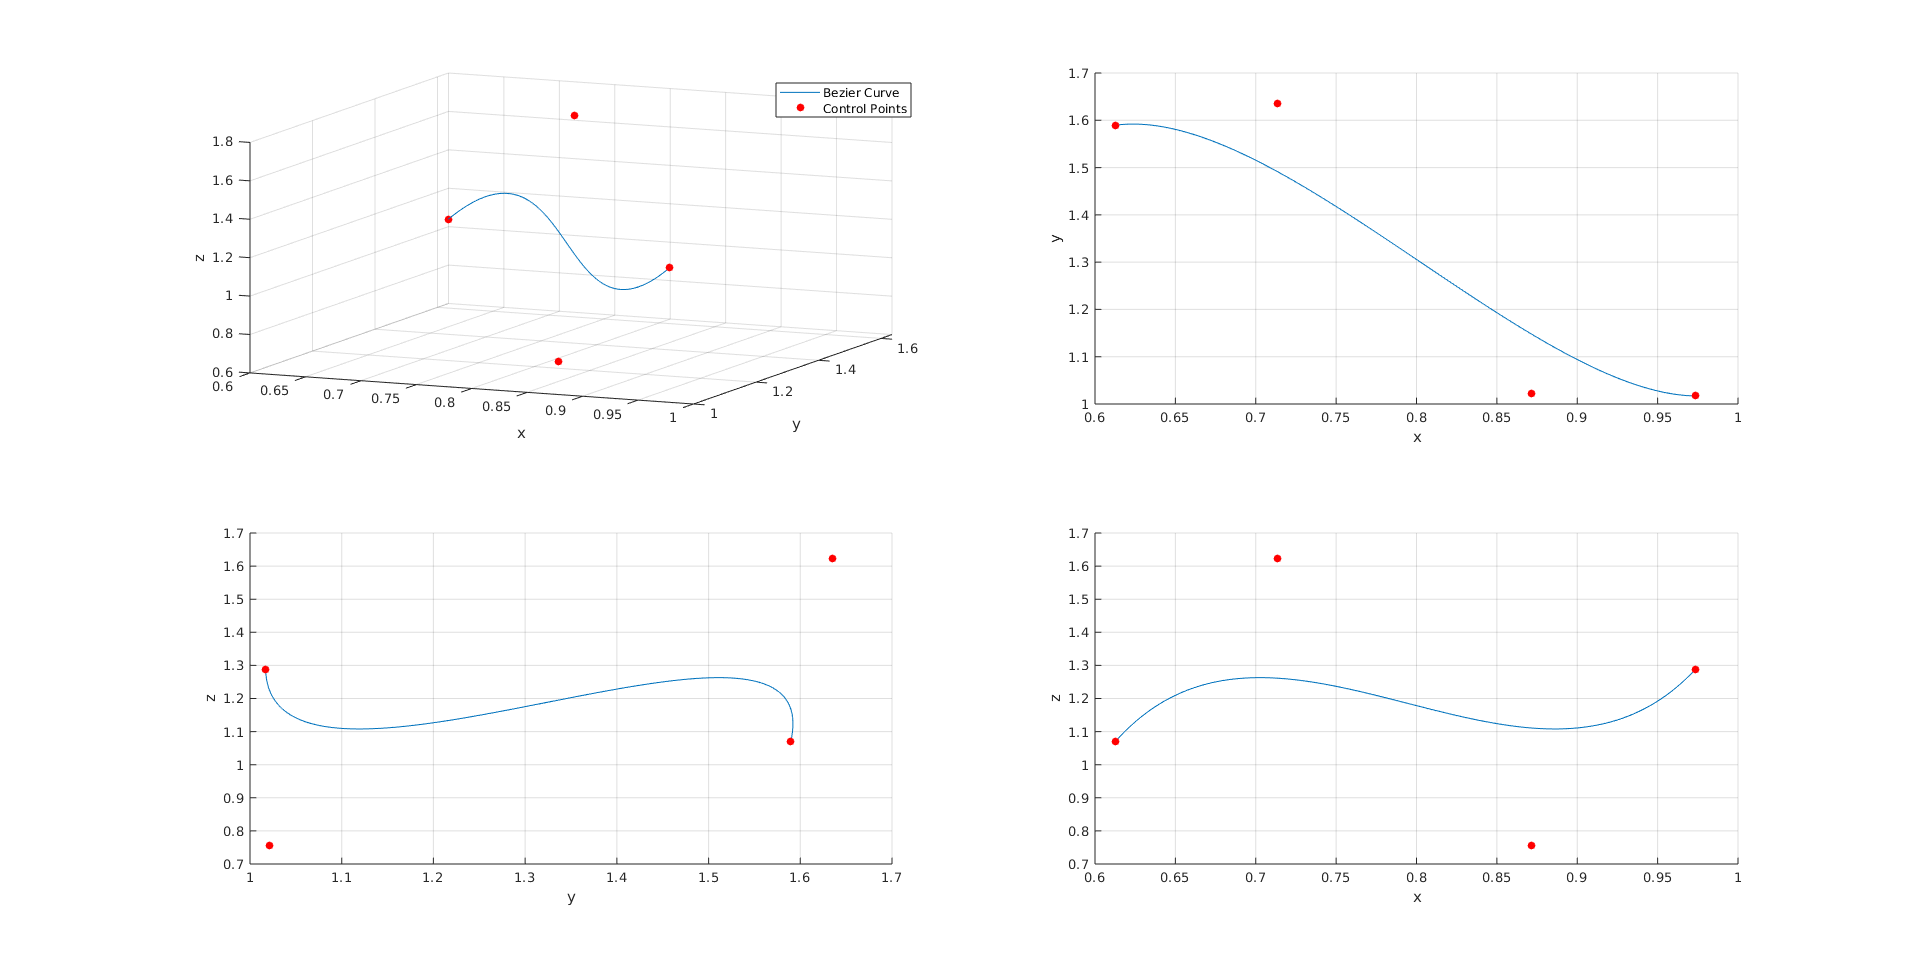
\includegraphics[width=0.7\textwidth]{images/bezier_path.png}\\
\caption{A cubic B\'ezier curve calculated and plotted in MATLAB} 
\end{figure}
\end{center}

A $k$-degree \textbf{B-Spline} curve defined by $n+1$ control points will consist of $n-k+1$ B\'ezier curves. For example if we want to construct a cubic B-Spline using 6 control points, then we will need to construct 
and connect together 3 B\'ezier curves.

\begin{center}
\begin{figure}[htbp]
\centering
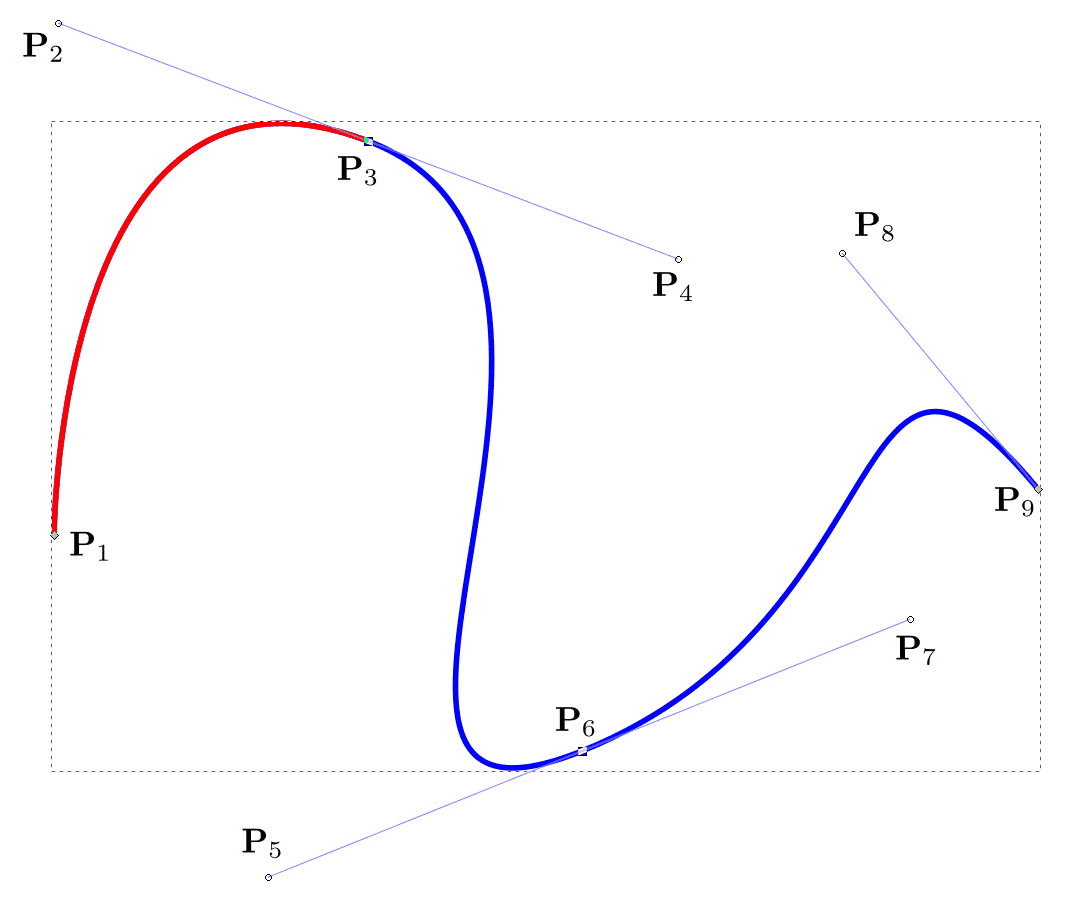
\includegraphics[width=0.7\textwidth]{images/b-spline-explanation.png}\\
\caption{B-Spline curve constructed from 3 B\'ezier curves. The first B\'ezier curve colored in red is a quadratic one and the following two are both cubic.} 
\label{b-spline-explanation}
\end{figure}
\end{center}

In most cases the B-Spline curves are constructed by starting from a quadratic B\'ezier curve, which is constructed from 3 control points and then all other 
parts of the curve are constructed from cubic B\'ezier curves, each constructed from 4 control points. As shown in figure \ref{b-spline-explanation}, the B-Spline 
curves do not pass from all control points. This means that if we have a path formed by a set of waypoints and we want the robot to pass from all of them, then 
in order to construct a B-Spline trajectory we will need additional intermediary points. The first and last points are part of the curve and the other control 
points are not. If no additional points can be calculated then the robot will not pass from all the points, which in some cases is also acceptable and useful. \\

One must notice also, in figure \ref{b-spline-explanation} for example, that some points must be colinear in order for the transition from one B\'ezier curve to another to be smooth, or equivalently 
the point where the two curves are connected to have a continuous derivative. For example in figure \ref{b-spline-explanation}, $\mathbf{P}_2, \mathbf{P}_3, \mathbf{P}_4$ must be colinear so that the 
derivative of the curve at $\mathbf{P}_3$ is continuous. In the same example one can also notice that if the distance of $\overrightarrow{\mathbf{P}_2\mathbf{P}_3}$ and $\overrightarrow{\mathbf{P}_3\mathbf{P}_4}$ 
is getting smaller then the curve at $\mathbf{P}_3$ is getting sharper and if these distances are $0$ then instead of a smooth curve we have a sharp corner and the curve has 
no longer a continuous derivative at $\mathbf{P}_3$. These two parameters; \textbf{3 colinear points} and the \textbf{distances of the two vectors} of these 3 colinear points can be very useful in designing 
B-Spline trajectories when we only have the waypoints available and not the extra control points required to construct the B\'ezier curves.\\

It is very important that the designed trajectory respects the joints angles' range. The robot arm may reach it's joint bounds and in order to 
continue executing the trajectory it will have to make a sudden jump to reset the angles. 
This could have serious side-effects for both the surgical task and thus the patient, as well as 
for the operating staff, who control the robot.

\begin{center}
\begin{figure}[htbp]
\centering
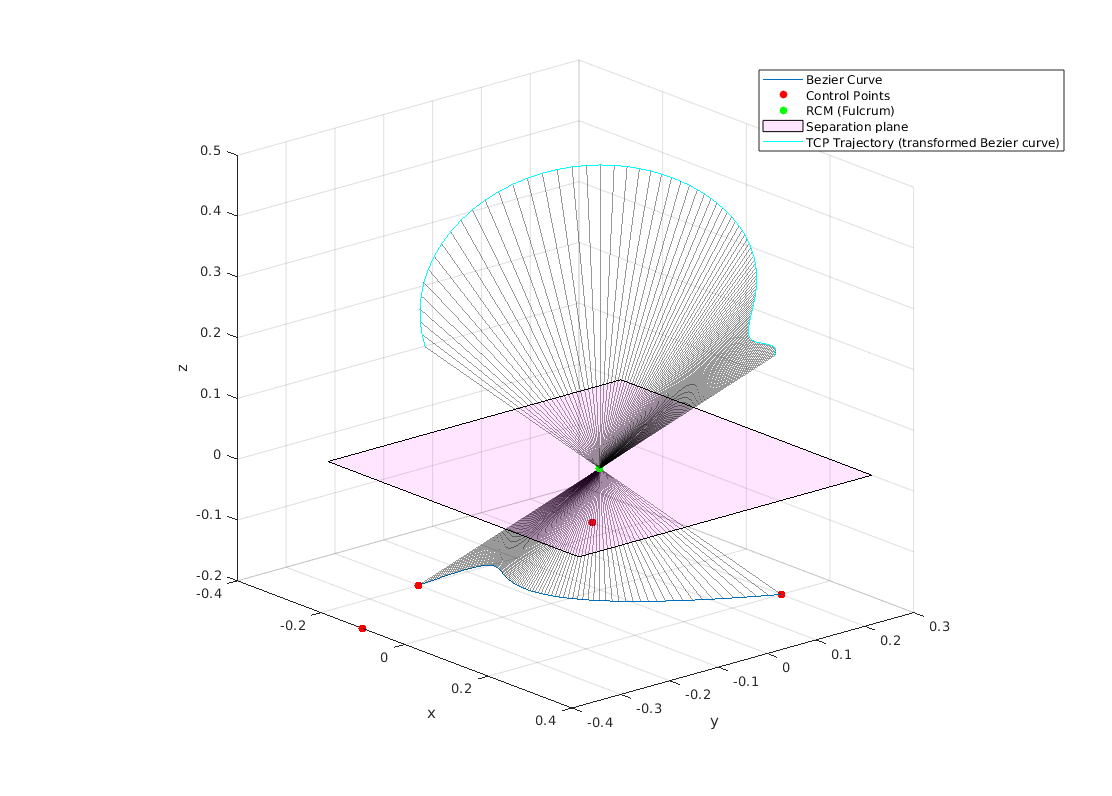
\includegraphics[width=0.7\textwidth]{images/rcm_trajectories/rcm_bezier_traj.png}\\
\caption{A B\'ezier curve trajectory and it's transformation via the Fulcrum Effect}
\end{figure}
\end{center}


\section{Trajectory planning in joint angles space}

\underline{Advantages of planning in Joint Space}
\begin{itemize}
\item Planning trajectories in Joint Space is \textbf{much faster in execution} than Task Space planning, because the Inverse Kinematics problem is solved for fewer points, only at the waypoints of the trajectory 
and not at the intermediate points (the points between the waypoints).
\item The actuators' motion is smoother
\end{itemize}

\underline{Disadvantages of planning in Joint Space}
\begin{itemize}
\item The interpolated intermediate points are not guaranteed to be collision-free.
\end{itemize}



\subsection{Polynomials of 5th order}
\label{section-polynomials-5}

Sometimes for a smooth trajectory between 2 consecutive path points, polynomials of higher degree are used. One such common family of polynomials are those of 5th degree with which we can specify the desired 
position, velocity, as well as acceleration at the beginning and at the end of the trajectory segment. This polynomial has the following closed form

\begin{equation}
q_i(t) = a_i + b_it + c_it^2 + d_it^3 + e_it^4 + f_it^5
\end{equation}

where
\begin{equation}
\begin{gathered}
q_i = q_i(t_i), \quad q_{i+1} = q_i(t_{i+1}) = q_{i+1}(t_{i+1}) \quad \textrm{and} \quad t_i \leq t \leq t_{i+1}
\end{gathered}
\end{equation}

The constants $a_i, b_i, \cdots, f_i$ are computed from the boundary conditions, i.e. the position, and its derivatives, evaluated at the beginning and at the end of the trajectory segment.

\begin{equation}
\label{polynomial5th-bound-conditions-eq}
\begin{aligned}
q_i ={}& a_i \\
q_{i+1} ={}& a_i + b_it_{i+1} + c_it_{i+1}^2 + d_it_{i+1}^3 + e_it_{i+1}^4 + f_it_{i+1}^5 \\
\dot{q}_i ={}& b_i \\ 
\dot{q}_{i+1} ={}& b_i + 2c_it_{i+1} + 3d_it_{i+1}^2 + 4e_it_{i+1}^3 + 5f_it_{i+1}^4 \\
\ddot{q}_i ={}& 2c_i \\
\ddot{q}_{i+1} ={}& 2c_i + 6d_it_{i+1} + 12e_it_{i+1}^2 + 20f_it_{i+1}^3
\end{aligned}
\end{equation}

Solving the system of boundary condition equations \ref{polynomial5th-bound-conditions-eq}, the solution for the constants is the following
\begin{equation}
\begin{aligned}
a_i ={}& q_i \\
b_i ={}& \dot{q}_i \\
c_i ={}& \frac{\ddot{q}_i}{2} \\
d_i ={}& \frac{20q_{i+1} - 20q_i - (8\dot{q}_{i+1} + 12\dot{q}_i)t_{i+1} - (3\ddot{q}_i - \ddot{q}_{i+1})t_{i+1}^2 }{2t_{i+1}^3} \\
e_i ={}& \frac{30q_i - 30q_{i+1} - (14\dot{q}_{i+1} + 16\dot{q}_i)t_{i+1} + (3\ddot{q}_i - 2\ddot{q}_{i+1})t_{i+1}^2}{2t_{i+1}^4} \\
f_i ={}& \frac{12q_{i+1} - 12q_i - (6\dot{q}_{i+1} + 6\dot{q}_i)t_{i+1} - (\ddot{q}_i - \ddot{q}_{i+1})t_{i+1}^2 }{2t_{i+1}^5}
\end{aligned}
\end{equation}


\subsection{Planning with velocity profiles}

\subsubsection{Trapezoid velocity profile - LSPB}

Trapezoid velocity profiles are a family of trajectories in motion control, that combines (blends) a linear segment with two parabolic segments. This type of trajectory is also known in the bibliography as 
Linear Segments with Parabolic Blends or LSPB. The equations of motions are studied in 3 intervals $[t_i, t_a], [t_a, t_d]$ and $[t_d, t_{i+1}]$ where $t_a = t_i + τ$ and $t_d = t_{i+1} - τ$ where $τ$ is 
the time duration for both the acceleration and deceleration phases (symmetric trapezoid profile). \\

For $t_i \leq t \leq t_a$ the equations of the trajectory are the following:

\begin{equation}
q_i(t) = c_0 + c_1t + c_2t^2, \quad c_0,c_1,c_2 \in \mathbb{R}
\end{equation}

\begin{equation}
\dot{q}_i(t) = c_1 + 2c_2t
\end{equation}

Using the initial conditions $q_i(0) = q_i$, $\dot{q}_i(0) = 0$ and $\dot{q}_i(t_a) = \dot{q}_{ic}$ we can solve for the constants $c_i$. $\dot{q}_{ic}$ is the desired constant velocity for the linear segment.
\begin{equation}
c_0 = q_i \quad \textrm{and} \quad c_1 = 0
\end{equation}

\[
\dot{q}_i + 2c_2t_a = \dot{q}_{ic}
\]

\begin{equation}
c_2 = \frac{\dot{q}_{ic}}{2t_a}
\end{equation}

The trajectory solution for $t_i \leq t \leq t_a$ is

\begin{equation}
\begin{aligned}
q_i(t) ={}& q_i + \frac{\dot{q}_{ic}}{2t_a}t^2 \\
\dot{q}_i(t) ={}& \frac{\dot{q}_{ic}}{t_a}t \\
\ddot{q}_i(t) ={}& \frac{\dot{q}_{ic}}{t_a} \\
\end{aligned}
\end{equation}

For $t_a \leq t \leq t_d$ the equations of the trajectory are the following:

\begin{equation}
q_i(t) = q_i(t_a) + \dot{q}_{ic}(t-t_a)
\end{equation}

Due to the symmetry of the trajectory, at half time the following equation must hold, that incorporates the 2 boundary conditions for the joint position
\begin{equation}
\label{eq:trap1}
q_i(t_{h}) = \frac{q_i + q_{i+1}}{2}, \quad \textrm{where} \quad t_h = \frac{t_{i+1} - t_i}{2}
\end{equation}
and
\begin{equation}
\label{eq:trap2}
q_i(t_{h}) = q_i(t_a) + \dot{q}_{ic}(t_h - t_a)
\end{equation}

Combining \ref{eq:trap1} and \ref{eq:trap2} the joint position at $t_a$ is
\begin{equation}
q_i(t_a) = \frac{q_i + q_{i+1}}{2} - \dot{q}_{ic}(t_h - t_a)
\end{equation}

The trajectory solution for $t_a \leq t \leq t_d$ is
\begin{equation}
\begin{aligned}
q_i(t) ={}& \frac{q_i + q_{i+1}}{2} - \dot{q}_{ic}(t_h - t_a) + \dot{q}_{ic}(t-t_a) \\
\dot{q}_i(t) ={}& \dot{q}_{ic} \\
\ddot{q}_i(t) ={}& 0 \\
\end{aligned}
\end{equation}

For $t_d \leq t \leq t_{i+1}$ the equations of the trajectory are similar to those of the first interval. Let $q_{i1}$ be the parabolic function of the first segment. From that the other 
parabolic segment will be calculated by mirroring $q_{i1}$ by the $t$-axis, shift to $t_{i+1}$ on the $t$-axis and translate by $q_{i+1} + q_i$ on the $y$-axis.

\begin{equation}
q_i(t) = -q_{i1}(t-t_{i+1}) + (q_{i+1} + q_i)
\end{equation}

The trajectory solution for $t_d \leq t \leq t_{i+1}$ is
\begin{equation}
\begin{aligned}
q_i(t) ={}& q_{i+1} - \frac{\dot{q}_{ic}}{2t_a}t^2 \\
\dot{q}_i(t) ={}& -\frac{\dot{q}_{ic}}{t_a}t \\
\ddot{q}_i(t) ={}& -\frac{\dot{q}_{ic}}{t_a} \\
\end{aligned}
\end{equation}

It is important to note that in order for the motion control using a trapezoid velocity profile to be feasible, the desired constant velocity $\dot{q}_{ic}$ must satisfy a velocity constraint. The constraint is 
calculated using the equations at time $t_a = t_i + τ$

\begin{equation}
q_i(t_a) = \frac{q_i + q_{i+1}}{2} - \dot{q}_{ic} \left( \frac{t_f}{2} - t_a \right) = q_i + \frac{\dot{q}_{ic}}{2t_a}t_a^2
\end{equation}
where $t_f/2 = t_h$

\begin{equation}
\frac{q_i + q_{i+1} - \dot{q}_{ic}t_f}{2} + \dot{q}_{ic}t_a = q_i + \frac{\dot{q}_{ic}}{2}t_a
\end{equation}

\begin{equation}
\frac{q_{i+1} - q_i - \dot{q}_{ic}t_f}{2} = -\frac{\dot{q}_{ic}}{2}t_a
\end{equation}

\begin{equation}
\label{eq:ta}
t_a = \frac{\dot{q}_{ic}t_f + q_i - q_{i+1}}{\dot{q}_{ic}}
\end{equation}

For the time constant $t_a$ the following inequalities must hold (to simplify calculations we consider the case where $t_i = 0$)

\begin{equation}
0 \leq t_a \leq \frac{t_f}{2} = t_h
\end{equation}

Substituting $t_a$ with \ref{eq:ta}
\begin{equation}
0 \leq \frac{\dot{q}_{ic}t_f + q_i - q_{i+1}}{\dot{q}_{ic}} \leq \frac{t_f}{2}
\end{equation}

\begin{equation}
0 \leq 2\dot{q}_{ic}t_f + 2(q_i-q_{i+1}) \leq \dot{q}_{ic}t_f
\end{equation}

\begin{equation}
-2\dot{q}_{ic}t_f \leq 2(q_i - q_{i+1}) \leq -\dot{q}_{ic}t_f
\end{equation}

\begin{equation}
- \frac{t_f}{q_i - q_{i+1}} \geq \frac{1}{\dot{q}_{ic}} \geq -\frac{t_f}{2(q_i - q_{i+1})}
\end{equation}

\begin{equation}
\frac{q_i - q_{i+1}}{t_f} \leq \dot{q}_{ic} \leq \frac{2(q_i - q_{i+1})}{t_f}
\end{equation}


\subsubsection{S-Curve velocity profile}

The s-curve trajectories introduce a cubic term to joint position polynomial, which has as a result the derivative of the acceleration, also known in the bibliography as jerk, to be non-zero. When introducing jerk
in the equations of motion, then we can no longer have discontinuities in the acceleration which means generating a smoother trajectory than the trapezoid profile's trajectory. The equations of motions are studied 
in 7 intervals $[t_i, t_a], [t_a, t_b], [t_b, t_c], [t_c, t_d], [t_d, t_e], [t_e, t_g]$ and $[t_g, t_{i+1}]$ where 

\begin{equation}
\begin{aligned}
t_a ={}& t_i + τ_1 \\
t_b ={}& t_i + τ_1 + τ_2 \\
t_c ={}& t_i + 2τ_1 + τ_2 \\
t_d ={}& t_{i+1} - 2τ_1 - τ_2 \\
t_e ={}& t_{i+1} - τ_1 - τ_2 \\
t_g ={}& t_{i+1} - τ_1 \\
\end{aligned}
\end{equation}

where $τ_1$ is the time duration for both the acceleration and deceleration phases (symmetric trapezoid acceleration profile) and $τ_2$ is the time duration of constant, non-zero acceleration. \\

For $t_i \leq t \leq t_a$ the equations of the trajectory are the following:

\begin{equation}
q_i(t) = c_0 + c_1t + c_2t^2 + c_3t^3, \quad c_0,c_1,c_2,c_3 \in \mathbb{R}
\end{equation}

\begin{equation}
\dot{q}_i(t) = c_1 + 2c_2t + 3c_3t^2
\end{equation}

\begin{equation}
\ddot{q}_i(t) = 2c_2t + 6c_3t
\end{equation}

Using the following initial conditions, 

\begin{equation}
q_i(0) = q_i, \quad \dot{q}_i(0) = 0, \quad \textrm{and} \quad \ddot{q}_i(0) = 0
\end{equation}

the constants $c_0,c_1$ and $c_2$ can be calculated

\begin{equation}
c_0 = q_i, \quad c_1 = 0, \quad \textrm{and} \quad c_2 = 0
\end{equation}

Using a desired acceleration $\ddot{q}_a$ at time $t_a = t_i + τ_1$, the constant $c_3$ can be calculated

\begin{equation}
q^{(4)}(t) = 6c_3 = J_a \quad \textrm{and} \quad J_a = \frac{\ddot{q}_a}{τ_1}
\end{equation}

The trajectory solution for $t_i \leq t \leq t_a = t_i + τ_1$ is
\begin{equation}
\begin{aligned}
q_i(t) ={}& q_i - \frac{\ddot{q}_{a}}{6τ_1}t^3 \\
\dot{q}_i(t) ={}& \frac{\ddot{q}_{a}}{2τ_1}t^2 \\
\ddot{q}_i(t) ={}& \frac{\ddot{q}_{a}}{τ_1}t \\
\end{aligned}
\end{equation}

The trajectory solution for $t_a \leq t \leq t_b$ is
\begin{equation}
\begin{aligned}
q_i(t) ={}& q_a + \dot{q}_a(t-t_a) + \frac{\ddot{q}_a}{2}(t-t_a)^2 \\
\dot{q}_i(t) ={}& \dot{q}_a + \ddot{q}_a(t-t_a) \\
\ddot{q}_i(t) ={}& \ddot{q}_a \\
\end{aligned}
\end{equation}

The trajectory solution for $t_b \leq t \leq t_c$ is
\begin{equation}
\begin{aligned}
q_i(t) ={}& q_b + \dot{q}_b(t-t_b) + \frac{\ddot{q}_a}{2}(t-t_b)^2 - \frac{\ddot{q}_a}{6τ_1}(t-t_b)^3 \\
\dot{q}_i(t) ={}& \dot{q}_β + \ddot{q}_a(t-t_b) - \frac{\ddot{q}_a}{2τ_1}(t-t_b)^2 \\
\ddot{q}_i(t) ={}& \ddot{q}_a - \frac{\ddot{q}_a}{τ_1}(t-t_b) \\
\end{aligned}
\end{equation}

The trajectory solution for $t_c \leq t \leq t_d$ is
\begin{equation}
\begin{aligned}
q_i(t) ={}& q_c + \dot{q}_c(t-t_c) \\
\dot{q}_i(t) ={}& \dot{q}_c \\
\ddot{q}_i(t) ={}& 0 \\
\end{aligned}
\end{equation}

The trajectory solution for $t_d \leq t \leq t_e$ is
\begin{equation}
\begin{aligned}
q_i(t) ={}& q_d + \dot{q}_c(t-t_d) - \frac{\ddot{q}_a}{6τ_1}(t-t_d)^3 \\
\dot{q}_i(t) ={}& \dot{q}_c - \frac{\ddot{q}_a}{2τ_1}(t-t_d)^2 \\
\ddot{q}_i(t) ={}& -\frac{\ddot{q}_a}{τ_1}(t-t_d) \\
\end{aligned}
\end{equation}

The trajectory solution for $t_e \leq t \leq t_g$ is
\begin{equation}
\begin{aligned}
q_i(t) ={}& q_e + \dot{q}_e(t-t_e) - \frac{\ddot{q}_a}{2}(t-t_e)^2 \\
\dot{q}_i(t) ={}& \dot{q}_e - \ddot{q}_a(t-t_e) \\
\ddot{q}_i(t) ={}& -\ddot{q}_a \\
\end{aligned}
\end{equation}

The trajectory solution for $t_g \leq t \leq t_{i+1}$ is
\begin{equation}
\begin{aligned}
q_i(t) ={}& q_g + \dot{q}_g(t-t_g) - \frac{\ddot{q}_a}{2}(t-t_g)^2 + \frac{\ddot{q}_a}{6τ_1}(t-t_g)^3 \\
\dot{q}_i(t) ={}& \dot{q}_g - \ddot{q}_a(t-t_g) + \frac{\ddot{q}_a}{2τ_1}(t-t_g)^2 \\
\ddot{q}_i(t) ={}& -\ddot{q}_a + \frac{\ddot{q}_a}{τ_1}(t-t_g) \\
\end{aligned}
\end{equation}

The equations of the s-curve profile trajectories can also be calculated numerically using integrals, which is however susceptible to small error accumulations. The integral trajectory solution for 
$t_k < t \leq t_{k+1}$ is
\begin{equation}
\begin{aligned}
q_k(t) ={}& q_k + \int_{t_k}^t \dot{q}_k(τ)dτ \\
\dot{q}_k(t) ={}& \dot{q}_k + \int_{t_k}^t \ddot{q}_k(τ)dτ \\
\ddot{q}_k(t) ={}& \ddot{q}_k + \int_{t_k}^t \dddot{q}_k(τ)dτ \\
\end{aligned}
\end{equation}

In order to better impose the boundary conditions for the start and end joint positions as well as fix any calculation errors, the following correction (normalization) formula can be used. 
Let $\tilde{q}_1$ and $\tilde{q}_2$ be the calculated start and end joint positions respectively. Then for each calculated joint position $\tilde{q}_k = q_i(t_k), \quad t_i \leq t_k \leq t_{i+1}$, 
the corrected joint position $q_k$ is calculated using the following equation

\begin{equation}
q_k = (\tilde{q}_k - q_1) \frac{q_2 - q_1}{\tilde{q}_2 - \tilde{q}_1} + q_1
\end{equation}


\begin{center}
\begin{figure}[htbp]
\centering
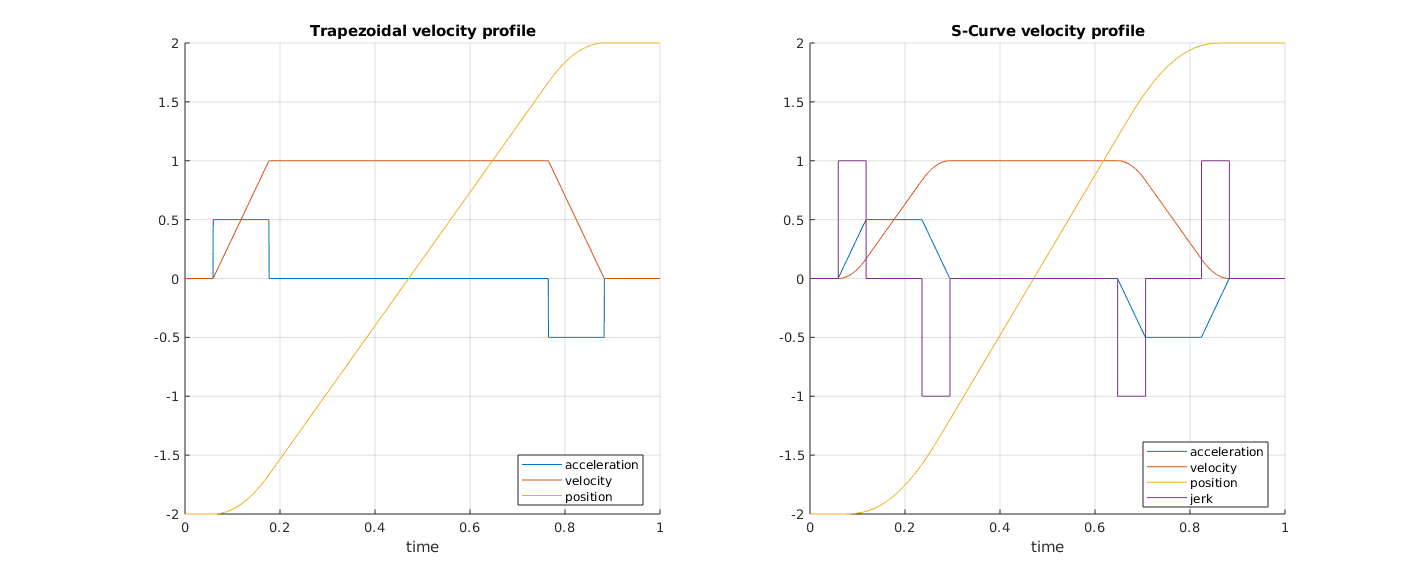
\includegraphics[width=0.7\textwidth]{images/vel-profiles.png}\\
\caption{Joint trajectory generated using velocity profiles. Calculated and plotted in MATLAB} 
\end{figure}
\end{center}


\subsubsection{Comparison of velocity profiles}

Both trapezoid and s-curve velocity profiles are widely used in industrial control systems, to design trajectories that are smooth and have a linear segment of constant velocity. Although both profiles are continuous in
position and velocity, the trapezoid profile does not have continuous acceleration and thus the generated trajectory is not smooth. These discontinuities in acceleration cause load oscillation or vibrations. This 
phenomenon can be easily observed in a cart-pendulum system like the one illustrated in \ref{cart-pendulum-passive-wrist-analogy}. The s-curve velocity profile can generate a smooth trajectory which at the start and end of 
the motion will have significantly less oscillation (overshoot in position). Experimental data showing this difference in motion (in one case there is overshoot/oscillation and in the other case there is not), for the cart-
pendulum system are available at the following article \url{https://www.pmdcorp.com/resources/type/articles/get/s-curve-profiles-deep-dive-article}. However, it is very important to note, that using smooth acceleration 
profiles in trajectories in the joint space $\mathbb{J}$ does not necessarily mean that the acceleration profile in the task space $\mathbb{P}$ will be equally smooth or any smooth at all due to the non-linear transformation 
between the spaces $\mathbb{J} \longleftrightarrow \mathbb{P}$ as well as the limits in the joint angles' ranges. This means that although smooth trajectories will cause less vibrations in the joint space, the vibrations/
oscillations are not necessarily avoided in the task space.

\begin{center}
\begin{figure}[htbp]
\centering
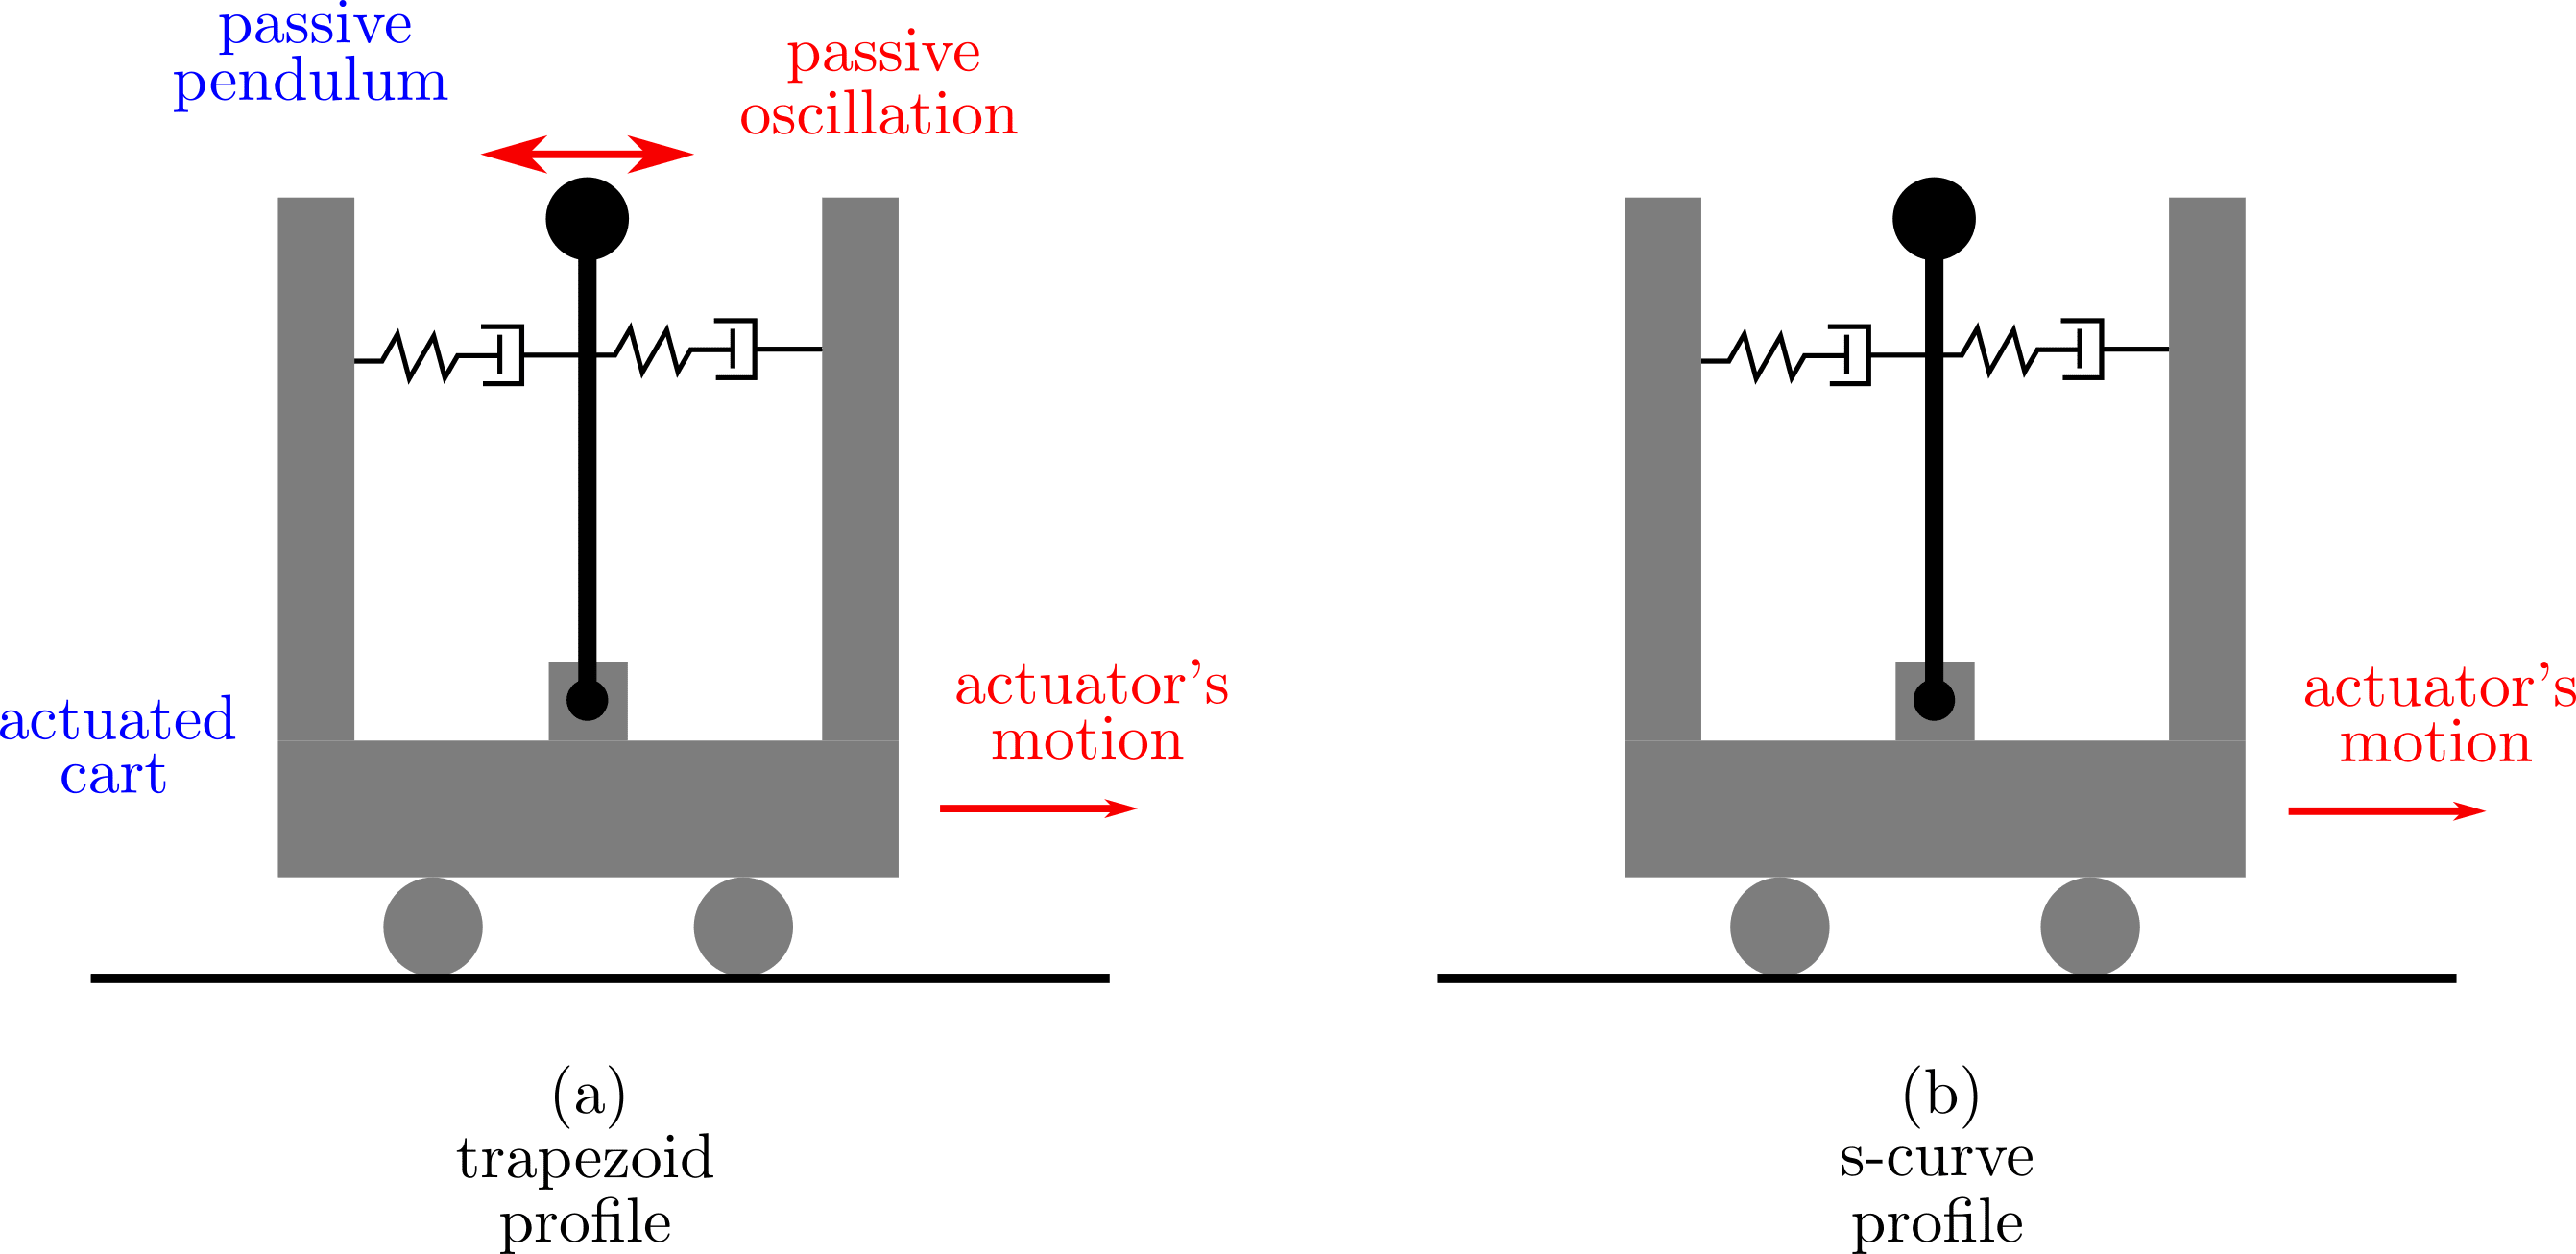
\includegraphics[width=0.7\textwidth]{images/cart-pendulum-passive-wrist-analogy.png}\\
\caption{Trapezoid vs s-curve velocity profiles applied to the cart-inverted-pendulum system.} 
\label{cart-pendulum-passive-wrist-analogy}
\end{figure}
\end{center}

The smoothness and absence of vibration/oscillation/overshoot in the point-to-point trajectory of a s-curve trajectory are especially useful in surgical robots that use passive wrists. A \textbf{passive wrist} is a mechanical 
device attached at the end-effector of a robot arm and it usually has 3 degrees of freedom which are passive, i.e. not actuated. Passive wrists are very useful in minimally-invasive surgery because they allow to use surgical 
tools (usually endoscopic cameras) that are inserted in the human body at the surgical site, through the trocar and the incision, without exerting much pressure. Passive wrists, however have the downside of passiveness 
(e.g. they can not be used for active tasks such as lifting an object, suturing etc.) and the difficulty in position control. Experimental data showing the overshoot and oscillation in position control of a
laparoscopic camera attached to a passive wrist, are available at figure 7 of article \cite{Bauzano2009ControlMF}.\\

An active-robot-passive-wrist system and the effect of trapezoid vs s-curve profile trajectories, can be studied using the analogous system of a cart-pendulum system as the one show in figure \ref{cart-pendulum-passive-wrist-analogy}. 
In figure \ref{cart-pendulum-passive-wrist-analogy} the cart is the actuated mechanism (the one that will have a motor) and the pendulum is the passive mechanism (i.e. the joint that attached the pendulum to the cart 
is not actuated). The pendulum is also attached to a spring-damper system to better simulate the oscillating response to sudden changes in acceleration/force. The pendulum, although not actuated, moves based on the sudden 
changes of motion of the cart. Using this analogy, the actuated cart can be thought of as the active robotic arm's end-effector and the passive pendulum can be thought of as the passive wrist which is attached to the 
end-effector.\\

Trapezoid and s-curve velocity profiles can be further extended and generalized using higher order s-curves where the jerk is also bounded and continuous. Based on each use case the higher order s-curves can be used to 
generated trajectories that are both controllable smooth and time-optimal. Higher order s-curve profiles can be found at \cite{Nguyen2008HigherOrderSCurves}.
